\documentclass[twoside]{book}

% Packages required by doxygen
\usepackage{calc}
\usepackage{doxygen}
\usepackage{graphicx}
\usepackage[utf8]{inputenc}
\usepackage{makeidx}
\usepackage{multicol}
\usepackage{multirow}
\usepackage{textcomp}
\usepackage[table]{xcolor}

% NLS support packages
\usepackage{hfont}

% Font selection
\usepackage[T1]{fontenc}
\usepackage{mathptmx}
\usepackage[scaled=.90]{helvet}
\usepackage{courier}
\usepackage{amssymb}
\usepackage{sectsty}
\renewcommand{\familydefault}{\sfdefault}
\allsectionsfont{%
  \fontseries{bc}\selectfont%
  \color{darkgray}%
}
\renewcommand{\DoxyLabelFont}{%
  \fontseries{bc}\selectfont%
  \color{darkgray}%
}

% Page & text layout
\usepackage{geometry}
\geometry{%
  a4paper,%
  top=2.5cm,%
  bottom=2.5cm,%
  left=2.5cm,%
  right=2.5cm%
}
\tolerance=750
\hfuzz=15pt
\hbadness=750
\setlength{\emergencystretch}{15pt}
\setlength{\parindent}{0cm}
\setlength{\parskip}{0.2cm}
\makeatletter
\renewcommand{\paragraph}{%
  \@startsection{paragraph}{4}{0ex}{-1.0ex}{1.0ex}{%
    \normalfont\normalsize\bfseries\SS@parafont%
  }%
}
\renewcommand{\subparagraph}{%
  \@startsection{subparagraph}{5}{0ex}{-1.0ex}{1.0ex}{%
    \normalfont\normalsize\bfseries\SS@subparafont%
  }%
}
\makeatother

% Headers & footers
\usepackage{fancyhdr}
\pagestyle{fancyplain}
\fancyhead[LE]{\fancyplain{}{\bfseries\thepage}}
\fancyhead[CE]{\fancyplain{}{}}
\fancyhead[RE]{\fancyplain{}{\bfseries\leftmark}}
\fancyhead[LO]{\fancyplain{}{\bfseries\rightmark}}
\fancyhead[CO]{\fancyplain{}{}}
\fancyhead[RO]{\fancyplain{}{\bfseries\thepage}}
\fancyfoot[LE]{\fancyplain{}{}}
\fancyfoot[CE]{\fancyplain{}{}}
\fancyfoot[RE]{\fancyplain{}{\bfseries\scriptsize 생성시간 \-: 수 9월 17 2014 06\-:28\-:37, 프로젝트명 \-: week8\-\_\-server, 생성자 \-:  Doxygen }}
\fancyfoot[LO]{\fancyplain{}{\bfseries\scriptsize 생성시간 \-: 수 9월 17 2014 06\-:28\-:37, 프로젝트명 \-: week8\-\_\-server, 생성자 \-:  Doxygen }}
\fancyfoot[CO]{\fancyplain{}{}}
\fancyfoot[RO]{\fancyplain{}{}}
\renewcommand{\footrulewidth}{0.4pt}
\renewcommand{\chaptermark}[1]{%
  \markboth{#1}{}%
}
\renewcommand{\sectionmark}[1]{%
  \markright{\thesection\ #1}%
}

% Indices & bibliography
\usepackage{natbib}
\usepackage[titles]{tocloft}
\setcounter{tocdepth}{3}
\setcounter{secnumdepth}{5}
\makeindex

% Hyperlinks (required, but should be loaded last)
\usepackage{ifpdf}
\ifpdf
  \usepackage[pdftex,pagebackref=true]{hyperref}
\else
  \usepackage[ps2pdf,pagebackref=true]{hyperref}
\fi
\hypersetup{%
  colorlinks=true,%
  linkcolor=blue,%
  citecolor=blue,%
  unicode%
}

% Custom commands
\newcommand{\clearemptydoublepage}{%
  \newpage{\pagestyle{empty}\cleardoublepage}%
}


%===== C O N T E N T S =====

\begin{document}

% Titlepage & ToC
\hypersetup{pageanchor=false}
\pagenumbering{roman}
\begin{titlepage}
\vspace*{7cm}
\begin{center}%
{\Large week8\-\_\-server }\\
\vspace*{1cm}
{\large 다음에 의해 생성됨 \-:  Doxygen 1.8.6}\\
\vspace*{0.5cm}
{\small 수 9월 17 2014 06:28:37}\\
\end{center}
\end{titlepage}
\clearemptydoublepage
\tableofcontents
\clearemptydoublepage
\pagenumbering{arabic}
\hypersetup{pageanchor=true}

%--- Begin generated contents ---
\chapter{네임스페이스 색인}
\section{패키지}
다음은 패키지들입니다. (가능한한 간략한 설명만을 보여줍니다) \-:\begin{DoxyCompactList}
\item\contentsline{section}{\hyperlink{namespaceweek8__server}{week8\-\_\-server} \\*Project package }{\pageref{namespaceweek8__server}}{}
\end{DoxyCompactList}

\chapter{계통도 색인}
\section{클래스 계통도}
이 상속 목록은 완전하진 않지만 알파벳순으로 대략적으로 정렬되어있습니다.\-:\begin{DoxyCompactList}
\item \contentsline{section}{week8\-\_\-server.\-Dispatcher}{\pageref{interfaceweek8__server_1_1_dispatcher}}{}
\begin{DoxyCompactList}
\item \contentsline{section}{week8\-\_\-server.\-Thread\-Per\-Dispatcher}{\pageref{classweek8__server_1_1_thread_per_dispatcher}}{}
\item \contentsline{section}{week8\-\_\-server.\-Thread\-Pool\-Dispatcher}{\pageref{classweek8__server_1_1_thread_pool_dispatcher}}{}
\end{DoxyCompactList}
\item \contentsline{section}{week8\-\_\-server.\-Event\-Handler}{\pageref{interfaceweek8__server_1_1_event_handler}}{}
\begin{DoxyCompactList}
\item \contentsline{section}{week8\-\_\-server.\-Stream\-Say\-Hello\-Event\-Handler}{\pageref{classweek8__server_1_1_stream_say_hello_event_handler}}{}
\item \contentsline{section}{week8\-\_\-server.\-Stream\-Update\-Profile\-Event\-Handler}{\pageref{classweek8__server_1_1_stream_update_profile_event_handler}}{}
\end{DoxyCompactList}
\item \contentsline{section}{week8\-\_\-server.\-Handler\-List\-Data}{\pageref{classweek8__server_1_1_handler_list_data}}{}
\item \contentsline{section}{week8\-\_\-server.\-Reactor}{\pageref{classweek8__server_1_1_reactor}}{}
\item Runnable\begin{DoxyCompactList}
\item \contentsline{section}{week8\-\_\-server.\-Demultiplexer}{\pageref{classweek8__server_1_1_demultiplexer}}{}
\end{DoxyCompactList}
\item \contentsline{section}{week8\-\_\-server.\-Server\-Initializer}{\pageref{classweek8__server_1_1_server_initializer}}{}
\item \contentsline{section}{week8\-\_\-server.\-Server\-List\-Data}{\pageref{classweek8__server_1_1_server_list_data}}{}
\item \contentsline{section}{week8\-\_\-server.\-Test\-Client}{\pageref{classweek8__server_1_1_test_client}}{}
\item Hash\-Map\begin{DoxyCompactList}
\item \contentsline{section}{week8\-\_\-server.\-Handle\-Map}{\pageref{classweek8__server_1_1_handle_map}}{}
\end{DoxyCompactList}
\end{DoxyCompactList}

\chapter{클래스 색인}
\section{클래스 목록}
다음은 클래스, 구조체, 공용체 그리고 인터페이스들입니다. (간략한 설명만을 보여줍니다) \-:\begin{DoxyCompactList}
\item\contentsline{section}{\hyperlink{classweek8__server_1_1_demultiplexer}{week8\-\_\-server.\-Demultiplexer} \\*Route request with header info to each handler }{\pageref{classweek8__server_1_1_demultiplexer}}{}
\item\contentsline{section}{\hyperlink{interfaceweek8__server_1_1_dispatcher}{week8\-\_\-server.\-Dispatcher} }{\pageref{interfaceweek8__server_1_1_dispatcher}}{}
\item\contentsline{section}{\hyperlink{interfaceweek8__server_1_1_event_handler}{week8\-\_\-server.\-Event\-Handler} }{\pageref{interfaceweek8__server_1_1_event_handler}}{}
\item\contentsline{section}{\hyperlink{classweek8__server_1_1_handle_map}{week8\-\_\-server.\-Handle\-Map} }{\pageref{classweek8__server_1_1_handle_map}}{}
\item\contentsline{section}{\hyperlink{classweek8__server_1_1_handler_list_data}{week8\-\_\-server.\-Handler\-List\-Data} }{\pageref{classweek8__server_1_1_handler_list_data}}{}
\item\contentsline{section}{\hyperlink{classweek8__server_1_1_reactor}{week8\-\_\-server.\-Reactor} \\*Method for reactor server, start / get,set handler }{\pageref{classweek8__server_1_1_reactor}}{}
\item\contentsline{section}{\hyperlink{classweek8__server_1_1_server_initializer}{week8\-\_\-server.\-Server\-Initializer} \\*Initializer class for Reactor-\/\-Thread using server }{\pageref{classweek8__server_1_1_server_initializer}}{}
\item\contentsline{section}{\hyperlink{classweek8__server_1_1_server_list_data}{week8\-\_\-server.\-Server\-List\-Data} }{\pageref{classweek8__server_1_1_server_list_data}}{}
\item\contentsline{section}{\hyperlink{classweek8__server_1_1_stream_say_hello_event_handler}{week8\-\_\-server.\-Stream\-Say\-Hello\-Event\-Handler} \\*Route request with header info to each handler }{\pageref{classweek8__server_1_1_stream_say_hello_event_handler}}{}
\item\contentsline{section}{\hyperlink{classweek8__server_1_1_stream_update_profile_event_handler}{week8\-\_\-server.\-Stream\-Update\-Profile\-Event\-Handler} \\*Route request with header info to each handler }{\pageref{classweek8__server_1_1_stream_update_profile_event_handler}}{}
\item\contentsline{section}{\hyperlink{classweek8__server_1_1_test_client}{week8\-\_\-server.\-Test\-Client} \\*Outputstream data for test }{\pageref{classweek8__server_1_1_test_client}}{}
\item\contentsline{section}{\hyperlink{classweek8__server_1_1_thread_per_dispatcher}{week8\-\_\-server.\-Thread\-Per\-Dispatcher} \\*\hyperlink{interfaceweek8__server_1_1_dispatcher}{Dispatcher} create thread for each stream }{\pageref{classweek8__server_1_1_thread_per_dispatcher}}{}
\item\contentsline{section}{\hyperlink{classweek8__server_1_1_thread_pool_dispatcher}{week8\-\_\-server.\-Thread\-Pool\-Dispatcher} }{\pageref{classweek8__server_1_1_thread_pool_dispatcher}}{}
\end{DoxyCompactList}

\chapter{파일 색인}
\section{파일 목록}
다음은 모든 파일에 대한 목록입니다. (간략한 설명만을 보여줍니다) \-:\begin{DoxyCompactList}
\item\contentsline{section}{src/week8\-\_\-server/\hyperlink{_demultiplexer_8java}{Demultiplexer.\-java} \\*Route request with header info to each handler }{\pageref{_demultiplexer_8java}}{}
\item\contentsline{section}{src/week8\-\_\-server/\hyperlink{_dispatcher_8java}{Dispatcher.\-java} \\*Dispatcher interface }{\pageref{_dispatcher_8java}}{}
\item\contentsline{section}{src/week8\-\_\-server/\hyperlink{_event_handler_8java}{Event\-Handler.\-java} \\*Event\-Handler interface }{\pageref{_event_handler_8java}}{}
\item\contentsline{section}{src/week8\-\_\-server/\hyperlink{_handle_map_8java}{Handle\-Map.\-java} \\*Handle\-Map for store handler }{\pageref{_handle_map_8java}}{}
\item\contentsline{section}{src/week8\-\_\-server/\hyperlink{_handler_list_data_8java}{Handler\-List\-Data.\-java} \\*Class for simpleframework }{\pageref{_handler_list_data_8java}}{}
\item\contentsline{section}{src/week8\-\_\-server/\hyperlink{_reactor_8java}{Reactor.\-java} \\*Method for reactor server, start / get,set handler }{\pageref{_reactor_8java}}{}
\item\contentsline{section}{src/week8\-\_\-server/\hyperlink{_server_initializer_8java}{Server\-Initializer.\-java} \\*Contains main method to run server / logger example }{\pageref{_server_initializer_8java}}{}
\item\contentsline{section}{src/week8\-\_\-server/\hyperlink{_server_list_data_8java}{Server\-List\-Data.\-java} \\*Class for simpleframework }{\pageref{_server_list_data_8java}}{}
\item\contentsline{section}{src/week8\-\_\-server/\hyperlink{_stream_say_hello_event_handler_8java}{Stream\-Say\-Hello\-Event\-Handler.\-java} }{\pageref{_stream_say_hello_event_handler_8java}}{}
\item\contentsline{section}{src/week8\-\_\-server/\hyperlink{_stream_update_profile_event_handler_8java}{Stream\-Update\-Profile\-Event\-Handler.\-java} \\*Handle request that header is 0x6001 }{\pageref{_stream_update_profile_event_handler_8java}}{}
\item\contentsline{section}{src/week8\-\_\-server/\hyperlink{_test_client_8java}{Test\-Client.\-java} \\*Outputstream data for test }{\pageref{_test_client_8java}}{}
\item\contentsline{section}{src/week8\-\_\-server/\hyperlink{_thread_per_dispatcher_8java}{Thread\-Per\-Dispatcher.\-java} \\*Dispatcher create thread for each stream }{\pageref{_thread_per_dispatcher_8java}}{}
\item\contentsline{section}{src/week8\-\_\-server/\hyperlink{_thread_pool_dispatcher_8java}{Thread\-Pool\-Dispatcher.\-java} \\*Dispatcher create thread pool and use for handle request }{\pageref{_thread_pool_dispatcher_8java}}{}
\end{DoxyCompactList}

\chapter{네임스페이스 문서화}
\hypertarget{namespaceweek8__server}{\section{week8\-\_\-server 패키지}
\label{namespaceweek8__server}\index{week8\-\_\-server@{week8\-\_\-server}}
}


project package  


\subsection*{클래스}
\begin{DoxyCompactItemize}
\item 
class \hyperlink{classweek8__server_1_1_demultiplexer}{Demultiplexer}
\begin{DoxyCompactList}\small\item\em route request with header info to each handler \end{DoxyCompactList}\item 
interface \hyperlink{interfaceweek8__server_1_1_dispatcher}{Dispatcher}
\item 
interface \hyperlink{interfaceweek8__server_1_1_event_handler}{Event\-Handler}
\item 
class \hyperlink{classweek8__server_1_1_handle_map}{Handle\-Map}
\item 
class \hyperlink{classweek8__server_1_1_handler_list_data}{Handler\-List\-Data}
\item 
class \hyperlink{classweek8__server_1_1_reactor}{Reactor}
\begin{DoxyCompactList}\small\item\em contains method for reactor server, start / get,set handler \end{DoxyCompactList}\item 
class \hyperlink{classweek8__server_1_1_server_initializer}{Server\-Initializer}
\begin{DoxyCompactList}\small\item\em Initializer class for Reactor-\/\-Thread using server. \end{DoxyCompactList}\item 
class \hyperlink{classweek8__server_1_1_server_list_data}{Server\-List\-Data}
\item 
class \hyperlink{classweek8__server_1_1_stream_say_hello_event_handler}{Stream\-Say\-Hello\-Event\-Handler}
\begin{DoxyCompactList}\small\item\em route request with header info to each handler \end{DoxyCompactList}\item 
class \hyperlink{classweek8__server_1_1_stream_update_profile_event_handler}{Stream\-Update\-Profile\-Event\-Handler}
\begin{DoxyCompactList}\small\item\em route request with header info to each handler \end{DoxyCompactList}\item 
class \hyperlink{classweek8__server_1_1_test_client}{Test\-Client}
\begin{DoxyCompactList}\small\item\em outputstream data for test \end{DoxyCompactList}\item 
class \hyperlink{classweek8__server_1_1_thread_per_dispatcher}{Thread\-Per\-Dispatcher}
\begin{DoxyCompactList}\small\item\em dispatcher create thread for each stream \end{DoxyCompactList}\item 
class \hyperlink{classweek8__server_1_1_thread_pool_dispatcher}{Thread\-Pool\-Dispatcher}
\end{DoxyCompactItemize}


\subsection{상세한 설명}
project package 
\chapter{클래스 문서화}
\hypertarget{classweek8__server_1_1_demultiplexer}{\section{week8\-\_\-server.\-Demultiplexer 클래스 참조}
\label{classweek8__server_1_1_demultiplexer}\index{week8\-\_\-server.\-Demultiplexer@{week8\-\_\-server.\-Demultiplexer}}
}


route request with header info to each handler  




week8\-\_\-server.\-Demultiplexer에 대한 상속 다이어그램 \-: 
\nopagebreak
\begin{figure}[H]
\begin{center}
\leavevmode
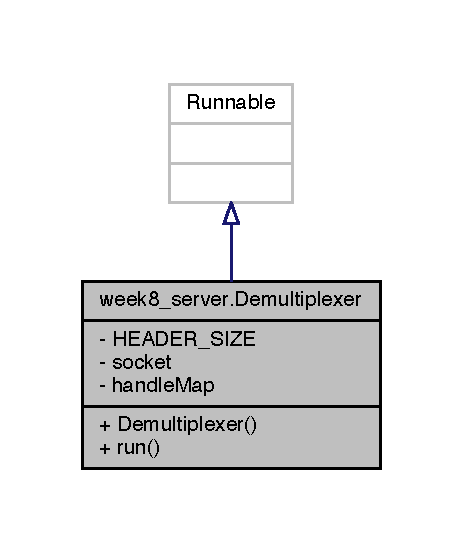
\includegraphics[width=222pt]{classweek8__server_1_1_demultiplexer__inherit__graph}
\end{center}
\end{figure}


week8\-\_\-server.\-Demultiplexer에 대한 협력 다이어그램\-:
\nopagebreak
\begin{figure}[H]
\begin{center}
\leavevmode
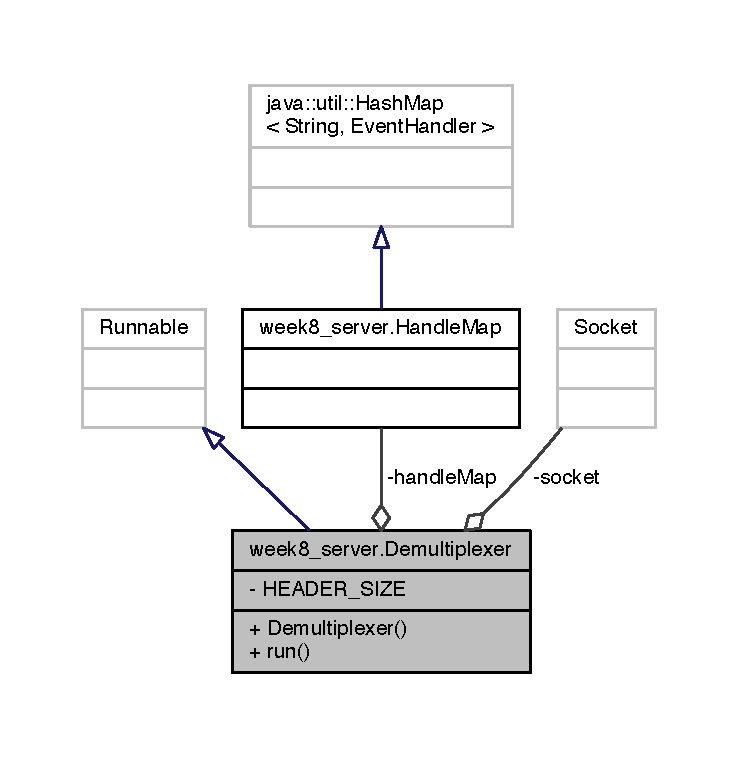
\includegraphics[width=350pt]{classweek8__server_1_1_demultiplexer__coll__graph}
\end{center}
\end{figure}
\subsection*{Public 멤버 함수}
\begin{DoxyCompactItemize}
\item 
\hyperlink{classweek8__server_1_1_demultiplexer_ad036466accbe99d2e8d1c09a50ecf70f}{Demultiplexer} (Socket \hyperlink{classweek8__server_1_1_demultiplexer_aa59bc55dc4eed3ea0247a8ea46913262}{socket}, \hyperlink{classweek8__server_1_1_handle_map}{Handle\-Map} \hyperlink{classweek8__server_1_1_demultiplexer_a9de8a7b062866296383729ba6e4ce0a1}{handle\-Map})
\item 
void \hyperlink{classweek8__server_1_1_demultiplexer_a5a09b3bc531ceb71fe22f1cadf3559c8}{run} ()
\end{DoxyCompactItemize}
\subsection*{Private 속성}
\begin{DoxyCompactItemize}
\item 
final int \hyperlink{classweek8__server_1_1_demultiplexer_a5240d883d891045d3cdf5f5497637eb1}{H\-E\-A\-D\-E\-R\-\_\-\-S\-I\-Z\-E} = 6
\item 
Socket \hyperlink{classweek8__server_1_1_demultiplexer_aa59bc55dc4eed3ea0247a8ea46913262}{socket}
\item 
\hyperlink{classweek8__server_1_1_handle_map}{Handle\-Map} \hyperlink{classweek8__server_1_1_demultiplexer_a9de8a7b062866296383729ba6e4ce0a1}{handle\-Map}
\end{DoxyCompactItemize}


\subsection{상세한 설명}
route request with header info to each handler 

\begin{DoxyDate}{날짜}
2014-\/09-\/17 
\end{DoxyDate}
\begin{DoxyAuthor}{작성자}
youngkim, \href{mailto:ky200223@nhnnext.org}{\tt ky200223@nhnnext.\-org}
\end{DoxyAuthor}
get request from socket, parse header then throw request to each header 

Demultiplexer.\-java 파일의 25 번째 라인에서 정의되었습니다.



\subsection{생성자 \& 소멸자 문서화}
\hypertarget{classweek8__server_1_1_demultiplexer_ad036466accbe99d2e8d1c09a50ecf70f}{\index{week8\-\_\-server\-::\-Demultiplexer@{week8\-\_\-server\-::\-Demultiplexer}!Demultiplexer@{Demultiplexer}}
\index{Demultiplexer@{Demultiplexer}!week8_server::Demultiplexer@{week8\-\_\-server\-::\-Demultiplexer}}
\subsubsection[{Demultiplexer}]{\setlength{\rightskip}{0pt plus 5cm}week8\-\_\-server.\-Demultiplexer.\-Demultiplexer (
\begin{DoxyParamCaption}
\item[{Socket}]{socket, }
\item[{{\bf Handle\-Map}}]{handle\-Map}
\end{DoxyParamCaption}
)}}\label{classweek8__server_1_1_demultiplexer_ad036466accbe99d2e8d1c09a50ecf70f}


Demultiplexer.\-java 파일의 32 번째 라인에서 정의되었습니다.


\begin{DoxyCode}
32                                                              \{
33         this.socket = \hyperlink{classweek8__server_1_1_demultiplexer_aa59bc55dc4eed3ea0247a8ea46913262}{socket};
34         this.handleMap = \hyperlink{classweek8__server_1_1_demultiplexer_a9de8a7b062866296383729ba6e4ce0a1}{handleMap};
35     \}
\end{DoxyCode}


\subsection{멤버 함수 문서화}
\hypertarget{classweek8__server_1_1_demultiplexer_a5a09b3bc531ceb71fe22f1cadf3559c8}{\index{week8\-\_\-server\-::\-Demultiplexer@{week8\-\_\-server\-::\-Demultiplexer}!run@{run}}
\index{run@{run}!week8_server::Demultiplexer@{week8\-\_\-server\-::\-Demultiplexer}}
\subsubsection[{run}]{\setlength{\rightskip}{0pt plus 5cm}void week8\-\_\-server.\-Demultiplexer.\-run (
\begin{DoxyParamCaption}
{}
\end{DoxyParamCaption}
)}}\label{classweek8__server_1_1_demultiplexer_a5a09b3bc531ceb71fe22f1cadf3559c8}


Demultiplexer.\-java 파일의 38 번째 라인에서 정의되었습니다.


\begin{DoxyCode}
38                       \{
39         \textcolor{keywordflow}{try} \{
40             InputStream is = socket.getInputStream();
41 
42             byte[] buffer = \textcolor{keyword}{new} byte[\hyperlink{classweek8__server_1_1_demultiplexer_a5240d883d891045d3cdf5f5497637eb1}{HEADER\_SIZE}];
43             is.read(buffer);
44             String header = \textcolor{keyword}{new} String(buffer);
45 
46             handleMap.get(header).handleEvent(is);
47 
48             socket.close();
49         \} \textcolor{keywordflow}{catch} (IOException e) \{
50             e.printStackTrace();
51         \}
52     \}
\end{DoxyCode}


\subsection{멤버 데이타 문서화}
\hypertarget{classweek8__server_1_1_demultiplexer_a9de8a7b062866296383729ba6e4ce0a1}{\index{week8\-\_\-server\-::\-Demultiplexer@{week8\-\_\-server\-::\-Demultiplexer}!handle\-Map@{handle\-Map}}
\index{handle\-Map@{handle\-Map}!week8_server::Demultiplexer@{week8\-\_\-server\-::\-Demultiplexer}}
\subsubsection[{handle\-Map}]{\setlength{\rightskip}{0pt plus 5cm}{\bf Handle\-Map} week8\-\_\-server.\-Demultiplexer.\-handle\-Map\hspace{0.3cm}{\ttfamily [private]}}}\label{classweek8__server_1_1_demultiplexer_a9de8a7b062866296383729ba6e4ce0a1}


Demultiplexer.\-java 파일의 30 번째 라인에서 정의되었습니다.

\hypertarget{classweek8__server_1_1_demultiplexer_a5240d883d891045d3cdf5f5497637eb1}{\index{week8\-\_\-server\-::\-Demultiplexer@{week8\-\_\-server\-::\-Demultiplexer}!H\-E\-A\-D\-E\-R\-\_\-\-S\-I\-Z\-E@{H\-E\-A\-D\-E\-R\-\_\-\-S\-I\-Z\-E}}
\index{H\-E\-A\-D\-E\-R\-\_\-\-S\-I\-Z\-E@{H\-E\-A\-D\-E\-R\-\_\-\-S\-I\-Z\-E}!week8_server::Demultiplexer@{week8\-\_\-server\-::\-Demultiplexer}}
\subsubsection[{H\-E\-A\-D\-E\-R\-\_\-\-S\-I\-Z\-E}]{\setlength{\rightskip}{0pt plus 5cm}final int week8\-\_\-server.\-Demultiplexer.\-H\-E\-A\-D\-E\-R\-\_\-\-S\-I\-Z\-E = 6\hspace{0.3cm}{\ttfamily [private]}}}\label{classweek8__server_1_1_demultiplexer_a5240d883d891045d3cdf5f5497637eb1}


Demultiplexer.\-java 파일의 27 번째 라인에서 정의되었습니다.

\hypertarget{classweek8__server_1_1_demultiplexer_aa59bc55dc4eed3ea0247a8ea46913262}{\index{week8\-\_\-server\-::\-Demultiplexer@{week8\-\_\-server\-::\-Demultiplexer}!socket@{socket}}
\index{socket@{socket}!week8_server::Demultiplexer@{week8\-\_\-server\-::\-Demultiplexer}}
\subsubsection[{socket}]{\setlength{\rightskip}{0pt plus 5cm}Socket week8\-\_\-server.\-Demultiplexer.\-socket\hspace{0.3cm}{\ttfamily [private]}}}\label{classweek8__server_1_1_demultiplexer_aa59bc55dc4eed3ea0247a8ea46913262}


Demultiplexer.\-java 파일의 29 번째 라인에서 정의되었습니다.



이 클래스에 대한 문서화 페이지는 다음의 파일로부터 생성되었습니다.\-:\begin{DoxyCompactItemize}
\item 
src/week8\-\_\-server/\hyperlink{_demultiplexer_8java}{Demultiplexer.\-java}\end{DoxyCompactItemize}

\hypertarget{interfaceweek8__server_1_1_dispatcher}{\section{week8\-\_\-server.\-Dispatcher 인터페이스 참조}
\label{interfaceweek8__server_1_1_dispatcher}\index{week8\-\_\-server.\-Dispatcher@{week8\-\_\-server.\-Dispatcher}}
}


week8\-\_\-server.\-Dispatcher에 대한 상속 다이어그램 \-: 
\nopagebreak
\begin{figure}[H]
\begin{center}
\leavevmode
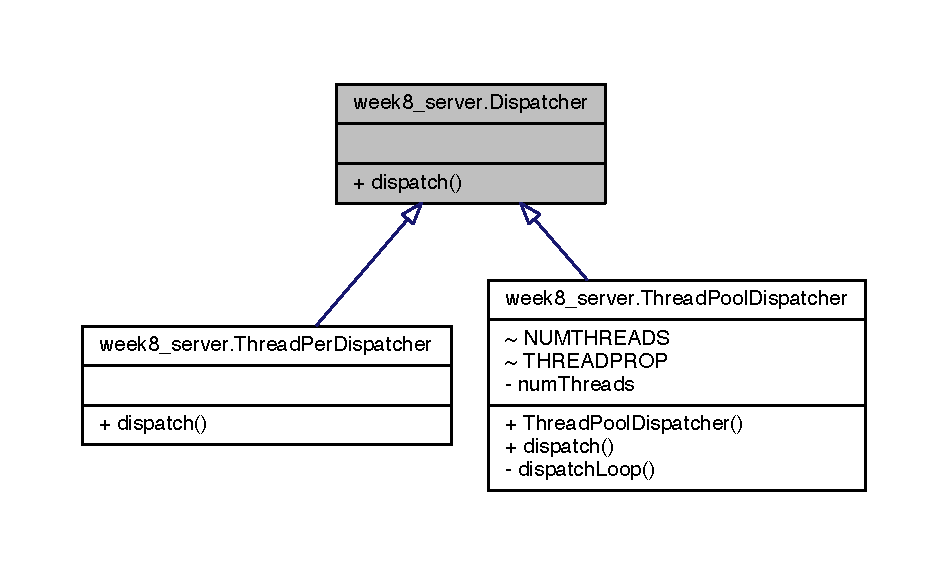
\includegraphics[width=350pt]{interfaceweek8__server_1_1_dispatcher__inherit__graph}
\end{center}
\end{figure}


week8\-\_\-server.\-Dispatcher에 대한 협력 다이어그램\-:
\nopagebreak
\begin{figure}[H]
\begin{center}
\leavevmode
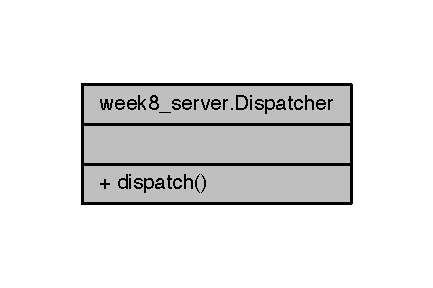
\includegraphics[width=208pt]{interfaceweek8__server_1_1_dispatcher__coll__graph}
\end{center}
\end{figure}
\subsection*{Public 멤버 함수}
\begin{DoxyCompactItemize}
\item 
void \hyperlink{interfaceweek8__server_1_1_dispatcher_a29b5387e03751725f89de08211e638b7}{dispatch} (Server\-Socket server\-Socket, \hyperlink{classweek8__server_1_1_handle_map}{Handle\-Map} handle\-Map)
\end{DoxyCompactItemize}


\subsection{상세한 설명}


Dispatcher.\-java 파일의 15 번째 라인에서 정의되었습니다.



\subsection{멤버 함수 문서화}
\hypertarget{interfaceweek8__server_1_1_dispatcher_a29b5387e03751725f89de08211e638b7}{\index{week8\-\_\-server\-::\-Dispatcher@{week8\-\_\-server\-::\-Dispatcher}!dispatch@{dispatch}}
\index{dispatch@{dispatch}!week8_server::Dispatcher@{week8\-\_\-server\-::\-Dispatcher}}
\subsubsection[{dispatch}]{\setlength{\rightskip}{0pt plus 5cm}void week8\-\_\-server.\-Dispatcher.\-dispatch (
\begin{DoxyParamCaption}
\item[{Server\-Socket}]{server\-Socket, }
\item[{{\bf Handle\-Map}}]{handle\-Map}
\end{DoxyParamCaption}
)}}\label{interfaceweek8__server_1_1_dispatcher_a29b5387e03751725f89de08211e638b7}


\hyperlink{classweek8__server_1_1_thread_per_dispatcher_acf253a1552859366b9420eb3ede8ea49}{week8\-\_\-server.\-Thread\-Per\-Dispatcher}에서 구현되었습니다.



이 인터페이스에 대한 문서화 페이지는 다음의 파일로부터 생성되었습니다.\-:\begin{DoxyCompactItemize}
\item 
src/week8\-\_\-server/\hyperlink{_dispatcher_8java}{Dispatcher.\-java}\end{DoxyCompactItemize}

\hypertarget{interfaceweek8__server_1_1_event_handler}{\section{week8\-\_\-server.\-Event\-Handler 인터페이스 참조}
\label{interfaceweek8__server_1_1_event_handler}\index{week8\-\_\-server.\-Event\-Handler@{week8\-\_\-server.\-Event\-Handler}}
}


week8\-\_\-server.\-Event\-Handler에 대한 상속 다이어그램 \-: 
\nopagebreak
\begin{figure}[H]
\begin{center}
\leavevmode
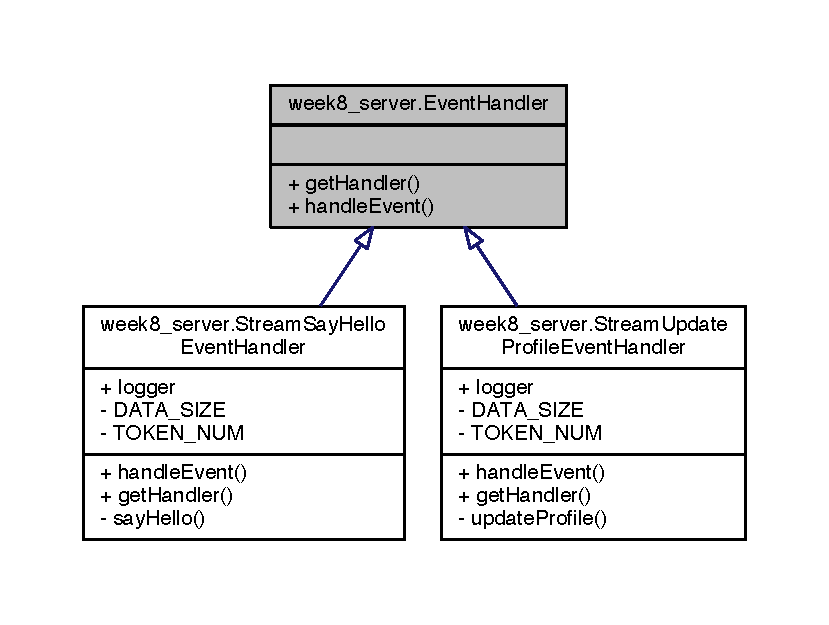
\includegraphics[width=350pt]{interfaceweek8__server_1_1_event_handler__inherit__graph}
\end{center}
\end{figure}


week8\-\_\-server.\-Event\-Handler에 대한 협력 다이어그램\-:
\nopagebreak
\begin{figure}[H]
\begin{center}
\leavevmode
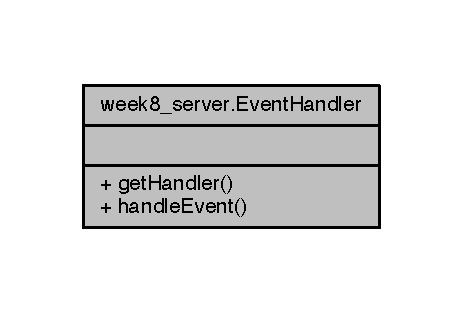
\includegraphics[width=222pt]{interfaceweek8__server_1_1_event_handler__coll__graph}
\end{center}
\end{figure}
\subsection*{Public 멤버 함수}
\begin{DoxyCompactItemize}
\item 
String \hyperlink{interfaceweek8__server_1_1_event_handler_a77b9a43471e25538de361dd0fff9478b}{get\-Handler} ()
\item 
void \hyperlink{interfaceweek8__server_1_1_event_handler_a24d2832c020ae27428c12be6d5277e51}{handle\-Event} (Input\-Stream is)
\end{DoxyCompactItemize}


\subsection{상세한 설명}


Event\-Handler.\-java 파일의 15 번째 라인에서 정의되었습니다.



\subsection{멤버 함수 문서화}
\hypertarget{interfaceweek8__server_1_1_event_handler_a77b9a43471e25538de361dd0fff9478b}{\index{week8\-\_\-server\-::\-Event\-Handler@{week8\-\_\-server\-::\-Event\-Handler}!get\-Handler@{get\-Handler}}
\index{get\-Handler@{get\-Handler}!week8_server::EventHandler@{week8\-\_\-server\-::\-Event\-Handler}}
\subsubsection[{get\-Handler}]{\setlength{\rightskip}{0pt plus 5cm}String week8\-\_\-server.\-Event\-Handler.\-get\-Handler (
\begin{DoxyParamCaption}
{}
\end{DoxyParamCaption}
)}}\label{interfaceweek8__server_1_1_event_handler_a77b9a43471e25538de361dd0fff9478b}


\hyperlink{classweek8__server_1_1_stream_say_hello_event_handler_a179e9b7dae2e32891de7dbc707e3d07e}{week8\-\_\-server.\-Stream\-Say\-Hello\-Event\-Handler}, \hyperlink{classweek8__server_1_1_stream_update_profile_event_handler_a0f5b195408dd8fb6b250ce8531a71f02}{week8\-\_\-server.\-Stream\-Update\-Profile\-Event\-Handler}에서 구현되었습니다.

\hypertarget{interfaceweek8__server_1_1_event_handler_a24d2832c020ae27428c12be6d5277e51}{\index{week8\-\_\-server\-::\-Event\-Handler@{week8\-\_\-server\-::\-Event\-Handler}!handle\-Event@{handle\-Event}}
\index{handle\-Event@{handle\-Event}!week8_server::EventHandler@{week8\-\_\-server\-::\-Event\-Handler}}
\subsubsection[{handle\-Event}]{\setlength{\rightskip}{0pt plus 5cm}void week8\-\_\-server.\-Event\-Handler.\-handle\-Event (
\begin{DoxyParamCaption}
\item[{Input\-Stream}]{is}
\end{DoxyParamCaption}
)}}\label{interfaceweek8__server_1_1_event_handler_a24d2832c020ae27428c12be6d5277e51}


\hyperlink{classweek8__server_1_1_stream_say_hello_event_handler_a2c2be02c3987ca818d6c09fd800d0f34}{week8\-\_\-server.\-Stream\-Say\-Hello\-Event\-Handler}, \hyperlink{classweek8__server_1_1_stream_update_profile_event_handler_a9cf985ef61eff5226bc397d72847abed}{week8\-\_\-server.\-Stream\-Update\-Profile\-Event\-Handler}에서 구현되었습니다.



이 인터페이스에 대한 문서화 페이지는 다음의 파일로부터 생성되었습니다.\-:\begin{DoxyCompactItemize}
\item 
src/week8\-\_\-server/\hyperlink{_event_handler_8java}{Event\-Handler.\-java}\end{DoxyCompactItemize}

\hypertarget{classweek8__server_1_1_handle_map}{\section{week8\-\_\-server.\-Handle\-Map 클래스 참조}
\label{classweek8__server_1_1_handle_map}\index{week8\-\_\-server.\-Handle\-Map@{week8\-\_\-server.\-Handle\-Map}}
}


week8\-\_\-server.\-Handle\-Map에 대한 상속 다이어그램 \-: 
\nopagebreak
\begin{figure}[H]
\begin{center}
\leavevmode
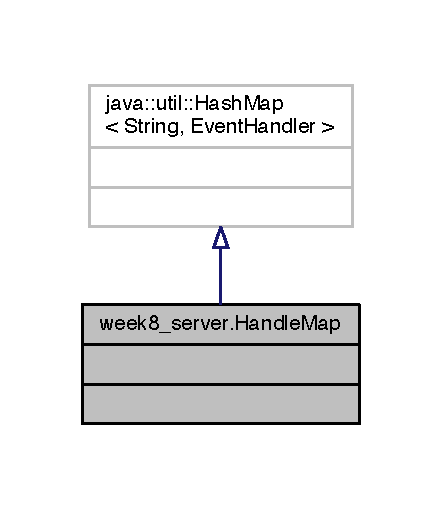
\includegraphics[width=212pt]{classweek8__server_1_1_handle_map__inherit__graph}
\end{center}
\end{figure}


week8\-\_\-server.\-Handle\-Map에 대한 협력 다이어그램\-:
\nopagebreak
\begin{figure}[H]
\begin{center}
\leavevmode
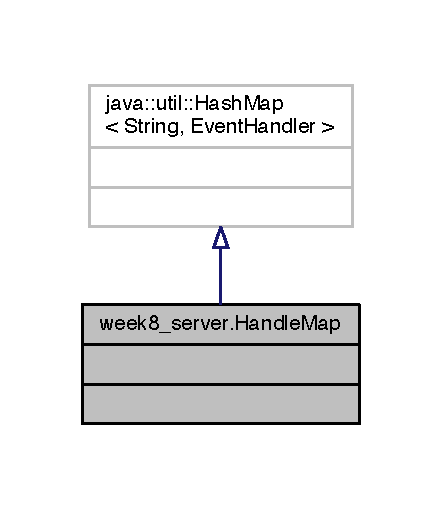
\includegraphics[width=212pt]{classweek8__server_1_1_handle_map__coll__graph}
\end{center}
\end{figure}


\subsection{상세한 설명}


Handle\-Map.\-java 파일의 15 번째 라인에서 정의되었습니다.



이 클래스에 대한 문서화 페이지는 다음의 파일로부터 생성되었습니다.\-:\begin{DoxyCompactItemize}
\item 
src/week8\-\_\-server/\hyperlink{_handle_map_8java}{Handle\-Map.\-java}\end{DoxyCompactItemize}

\hypertarget{classweek8__server_1_1_handler_list_data}{\section{week8\-\_\-server.\-Handler\-List\-Data 클래스 참조}
\label{classweek8__server_1_1_handler_list_data}\index{week8\-\_\-server.\-Handler\-List\-Data@{week8\-\_\-server.\-Handler\-List\-Data}}
}


week8\-\_\-server.\-Handler\-List\-Data에 대한 협력 다이어그램\-:
\nopagebreak
\begin{figure}[H]
\begin{center}
\leavevmode
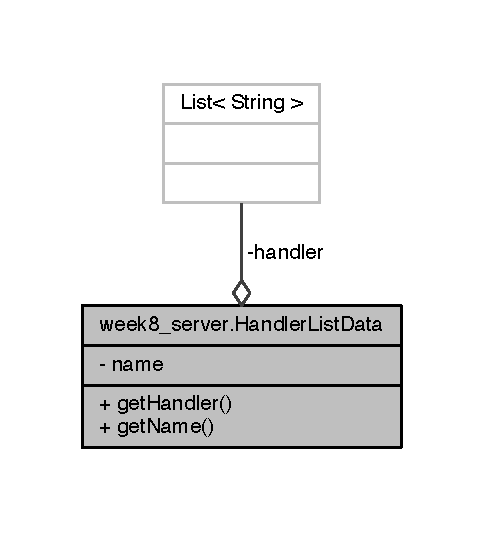
\includegraphics[width=232pt]{classweek8__server_1_1_handler_list_data__coll__graph}
\end{center}
\end{figure}
\subsection*{Public 멤버 함수}
\begin{DoxyCompactItemize}
\item 
List$<$ String $>$ \hyperlink{classweek8__server_1_1_handler_list_data_a1f90cf96677728ec88e603b59ae80e8e}{get\-Handler} ()
\item 
String \hyperlink{classweek8__server_1_1_handler_list_data_aa7ac90f82d504b25610eb401c729f57d}{get\-Name} ()
\end{DoxyCompactItemize}
\subsection*{Private 속성}
\begin{DoxyCompactItemize}
\item 
List$<$ String $>$ \hyperlink{classweek8__server_1_1_handler_list_data_a6905ecd2a867500c1096d5543b36bb91}{handler}
\item 
String \hyperlink{classweek8__server_1_1_handler_list_data_a6b207124eddb629f42eb688e7e107df1}{name}
\end{DoxyCompactItemize}


\subsection{상세한 설명}


Handler\-List\-Data.\-java 파일의 18 번째 라인에서 정의되었습니다.



\subsection{멤버 함수 문서화}
\hypertarget{classweek8__server_1_1_handler_list_data_a1f90cf96677728ec88e603b59ae80e8e}{\index{week8\-\_\-server\-::\-Handler\-List\-Data@{week8\-\_\-server\-::\-Handler\-List\-Data}!get\-Handler@{get\-Handler}}
\index{get\-Handler@{get\-Handler}!week8_server::HandlerListData@{week8\-\_\-server\-::\-Handler\-List\-Data}}
\subsubsection[{get\-Handler}]{\setlength{\rightskip}{0pt plus 5cm}List$<$String$>$ week8\-\_\-server.\-Handler\-List\-Data.\-get\-Handler (
\begin{DoxyParamCaption}
{}
\end{DoxyParamCaption}
)}}\label{classweek8__server_1_1_handler_list_data_a1f90cf96677728ec88e603b59ae80e8e}


Handler\-List\-Data.\-java 파일의 25 번째 라인에서 정의되었습니다.


\begin{DoxyCode}
25                                      \{
26         \textcolor{keywordflow}{return} \hyperlink{classweek8__server_1_1_handler_list_data_a6905ecd2a867500c1096d5543b36bb91}{handler};
27     \}
\end{DoxyCode}
\hypertarget{classweek8__server_1_1_handler_list_data_aa7ac90f82d504b25610eb401c729f57d}{\index{week8\-\_\-server\-::\-Handler\-List\-Data@{week8\-\_\-server\-::\-Handler\-List\-Data}!get\-Name@{get\-Name}}
\index{get\-Name@{get\-Name}!week8_server::HandlerListData@{week8\-\_\-server\-::\-Handler\-List\-Data}}
\subsubsection[{get\-Name}]{\setlength{\rightskip}{0pt plus 5cm}String week8\-\_\-server.\-Handler\-List\-Data.\-get\-Name (
\begin{DoxyParamCaption}
{}
\end{DoxyParamCaption}
)}}\label{classweek8__server_1_1_handler_list_data_aa7ac90f82d504b25610eb401c729f57d}


Handler\-List\-Data.\-java 파일의 29 번째 라인에서 정의되었습니다.


\begin{DoxyCode}
29                             \{
30         \textcolor{keywordflow}{return} \hyperlink{classweek8__server_1_1_handler_list_data_a6b207124eddb629f42eb688e7e107df1}{name};
31     \}
\end{DoxyCode}


\subsection{멤버 데이타 문서화}
\hypertarget{classweek8__server_1_1_handler_list_data_a6905ecd2a867500c1096d5543b36bb91}{\index{week8\-\_\-server\-::\-Handler\-List\-Data@{week8\-\_\-server\-::\-Handler\-List\-Data}!handler@{handler}}
\index{handler@{handler}!week8_server::HandlerListData@{week8\-\_\-server\-::\-Handler\-List\-Data}}
\subsubsection[{handler}]{\setlength{\rightskip}{0pt plus 5cm}List$<$String$>$ week8\-\_\-server.\-Handler\-List\-Data.\-handler\hspace{0.3cm}{\ttfamily [private]}}}\label{classweek8__server_1_1_handler_list_data_a6905ecd2a867500c1096d5543b36bb91}


Handler\-List\-Data.\-java 파일의 20 번째 라인에서 정의되었습니다.

\hypertarget{classweek8__server_1_1_handler_list_data_a6b207124eddb629f42eb688e7e107df1}{\index{week8\-\_\-server\-::\-Handler\-List\-Data@{week8\-\_\-server\-::\-Handler\-List\-Data}!name@{name}}
\index{name@{name}!week8_server::HandlerListData@{week8\-\_\-server\-::\-Handler\-List\-Data}}
\subsubsection[{name}]{\setlength{\rightskip}{0pt plus 5cm}String week8\-\_\-server.\-Handler\-List\-Data.\-name\hspace{0.3cm}{\ttfamily [private]}}}\label{classweek8__server_1_1_handler_list_data_a6b207124eddb629f42eb688e7e107df1}


Handler\-List\-Data.\-java 파일의 23 번째 라인에서 정의되었습니다.



이 클래스에 대한 문서화 페이지는 다음의 파일로부터 생성되었습니다.\-:\begin{DoxyCompactItemize}
\item 
src/week8\-\_\-server/\hyperlink{_handler_list_data_8java}{Handler\-List\-Data.\-java}\end{DoxyCompactItemize}

\hypertarget{classweek8__server_1_1_reactor}{\section{week8\-\_\-server.\-Reactor 클래스 참조}
\label{classweek8__server_1_1_reactor}\index{week8\-\_\-server.\-Reactor@{week8\-\_\-server.\-Reactor}}
}


contains method for reactor server, start / get,set handler  




week8\-\_\-server.\-Reactor에 대한 협력 다이어그램\-:
\nopagebreak
\begin{figure}[H]
\begin{center}
\leavevmode
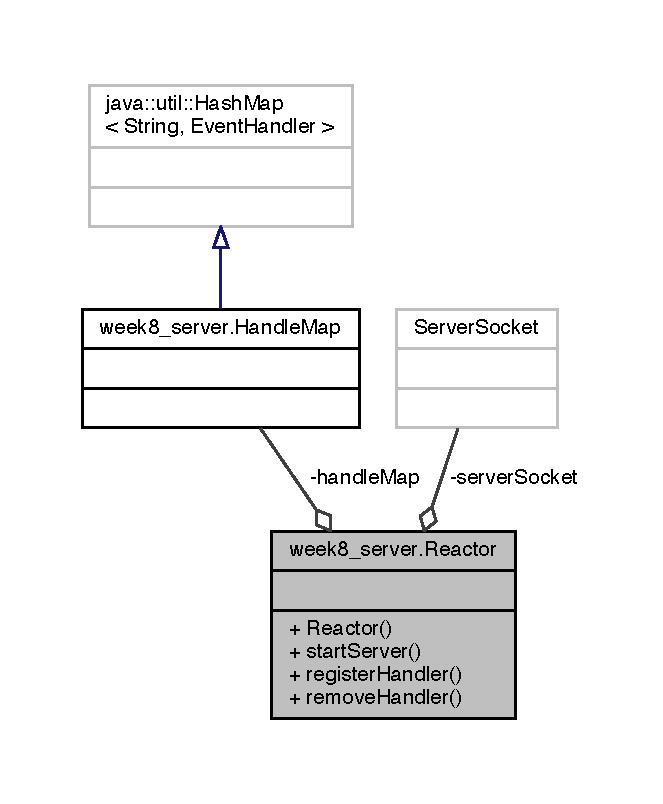
\includegraphics[width=318pt]{classweek8__server_1_1_reactor__coll__graph}
\end{center}
\end{figure}
\subsection*{Public 멤버 함수}
\begin{DoxyCompactItemize}
\item 
\hyperlink{classweek8__server_1_1_reactor_a1aaf09065cb067bad05bb829c7f2eb3e}{Reactor} (int port)
\begin{DoxyCompactList}\small\item\em init variable for server \end{DoxyCompactList}\item 
void \hyperlink{classweek8__server_1_1_reactor_a8dfd45d29257ccfd68f44425f1f4bc1d}{start\-Server} ()
\begin{DoxyCompactList}\small\item\em start\-Server \end{DoxyCompactList}\item 
void \hyperlink{classweek8__server_1_1_reactor_a798e0b09e61056876c94df493b6d9cc9}{register\-Handler} (\hyperlink{interfaceweek8__server_1_1_event_handler}{Event\-Handler} handler)
\begin{DoxyCompactList}\small\item\em register Handler \end{DoxyCompactList}\item 
void \hyperlink{classweek8__server_1_1_reactor_a6fdcf080ba274be3c539f00c7c87cd97}{remove\-Handler} (\hyperlink{interfaceweek8__server_1_1_event_handler}{Event\-Handler} handler)
\begin{DoxyCompactList}\small\item\em remove Handler \end{DoxyCompactList}\end{DoxyCompactItemize}
\subsection*{Private 속성}
\begin{DoxyCompactItemize}
\item 
Server\-Socket \hyperlink{classweek8__server_1_1_reactor_a0ccdb32c43af4ff402db7cdf9991492b}{server\-Socket}
\item 
\hyperlink{classweek8__server_1_1_handle_map}{Handle\-Map} \hyperlink{classweek8__server_1_1_reactor_a8ba93454e7dbe329e3fb503b94b5240e}{handle\-Map}
\end{DoxyCompactItemize}


\subsection{상세한 설명}
contains method for reactor server, start / get,set handler 

\begin{DoxyDate}{날짜}
2014-\/09-\/17 
\end{DoxyDate}
\begin{DoxyAuthor}{작성자}
youngkim, \href{mailto:ky200223@nhnnext.org}{\tt ky200223@nhnnext.\-org}
\end{DoxyAuthor}
create handle\-Map/open Server\-Socket, manage handler\-Event 

Reactor.\-java 파일의 23 번째 라인에서 정의되었습니다.



\subsection{생성자 \& 소멸자 문서화}
\hypertarget{classweek8__server_1_1_reactor_a1aaf09065cb067bad05bb829c7f2eb3e}{\index{week8\-\_\-server\-::\-Reactor@{week8\-\_\-server\-::\-Reactor}!Reactor@{Reactor}}
\index{Reactor@{Reactor}!week8_server::Reactor@{week8\-\_\-server\-::\-Reactor}}
\subsubsection[{Reactor}]{\setlength{\rightskip}{0pt plus 5cm}week8\-\_\-server.\-Reactor.\-Reactor (
\begin{DoxyParamCaption}
\item[{int}]{port}
\end{DoxyParamCaption}
)}}\label{classweek8__server_1_1_reactor_a1aaf09065cb067bad05bb829c7f2eb3e}


init variable for server 

create handle\-Map, open Server\-Socket 
\begin{DoxyParams}{매개변수}
{\em port} & \\
\hline
\end{DoxyParams}
\begin{DoxyReturn}{반환값}
none 
\end{DoxyReturn}


Reactor.\-java 파일의 33 번째 라인에서 정의되었습니다.


\begin{DoxyCode}
33                              \{
34         \hyperlink{classweek8__server_1_1_reactor_a8ba93454e7dbe329e3fb503b94b5240e}{handleMap} = \textcolor{keyword}{new} HandleMap();
35         \textcolor{keywordflow}{try} \{
36             \hyperlink{classweek8__server_1_1_reactor_a0ccdb32c43af4ff402db7cdf9991492b}{serverSocket} = \textcolor{keyword}{new} ServerSocket(port);
37         \} \textcolor{keywordflow}{catch} (IOException e) \{
38             e.printStackTrace();
39         \}
40     \}
\end{DoxyCode}


\subsection{멤버 함수 문서화}
\hypertarget{classweek8__server_1_1_reactor_a798e0b09e61056876c94df493b6d9cc9}{\index{week8\-\_\-server\-::\-Reactor@{week8\-\_\-server\-::\-Reactor}!register\-Handler@{register\-Handler}}
\index{register\-Handler@{register\-Handler}!week8_server::Reactor@{week8\-\_\-server\-::\-Reactor}}
\subsubsection[{register\-Handler}]{\setlength{\rightskip}{0pt plus 5cm}void week8\-\_\-server.\-Reactor.\-register\-Handler (
\begin{DoxyParamCaption}
\item[{{\bf Event\-Handler}}]{handler}
\end{DoxyParamCaption}
)}}\label{classweek8__server_1_1_reactor_a798e0b09e61056876c94df493b6d9cc9}


register Handler 

register Handler at \hyperlink{classweek8__server_1_1_handle_map}{Handle\-Map} 
\begin{DoxyParams}{매개변수}
{\em handler} & \\
\hline
\end{DoxyParams}
\begin{DoxyReturn}{반환값}
none 
\end{DoxyReturn}


Reactor.\-java 파일의 61 번째 라인에서 정의되었습니다.


\begin{DoxyCode}
61                                                       \{
62         handleMap.put(handler.getHandler(), handler);
63     \}
\end{DoxyCode}
\hypertarget{classweek8__server_1_1_reactor_a6fdcf080ba274be3c539f00c7c87cd97}{\index{week8\-\_\-server\-::\-Reactor@{week8\-\_\-server\-::\-Reactor}!remove\-Handler@{remove\-Handler}}
\index{remove\-Handler@{remove\-Handler}!week8_server::Reactor@{week8\-\_\-server\-::\-Reactor}}
\subsubsection[{remove\-Handler}]{\setlength{\rightskip}{0pt plus 5cm}void week8\-\_\-server.\-Reactor.\-remove\-Handler (
\begin{DoxyParamCaption}
\item[{{\bf Event\-Handler}}]{handler}
\end{DoxyParamCaption}
)}}\label{classweek8__server_1_1_reactor_a6fdcf080ba274be3c539f00c7c87cd97}


remove Handler 

remove Handler at \hyperlink{classweek8__server_1_1_handle_map}{Handle\-Map} 
\begin{DoxyParams}{매개변수}
{\em handler} & \\
\hline
\end{DoxyParams}
\begin{DoxyReturn}{반환값}
none 
\end{DoxyReturn}


Reactor.\-java 파일의 71 번째 라인에서 정의되었습니다.


\begin{DoxyCode}
71                                                     \{
72         handleMap.remove(handler.getHandler());
73     \}
\end{DoxyCode}
\hypertarget{classweek8__server_1_1_reactor_a8dfd45d29257ccfd68f44425f1f4bc1d}{\index{week8\-\_\-server\-::\-Reactor@{week8\-\_\-server\-::\-Reactor}!start\-Server@{start\-Server}}
\index{start\-Server@{start\-Server}!week8_server::Reactor@{week8\-\_\-server\-::\-Reactor}}
\subsubsection[{start\-Server}]{\setlength{\rightskip}{0pt plus 5cm}void week8\-\_\-server.\-Reactor.\-start\-Server (
\begin{DoxyParamCaption}
{}
\end{DoxyParamCaption}
)}}\label{classweek8__server_1_1_reactor_a8dfd45d29257ccfd68f44425f1f4bc1d}


start\-Server 

start dispatch 
\begin{DoxyParams}{매개변수}
{\em none} & \\
\hline
\end{DoxyParams}
\begin{DoxyReturn}{반환값}
none 
\end{DoxyReturn}


Reactor.\-java 파일의 48 번째 라인에서 정의되었습니다.


\begin{DoxyCode}
48                               \{
49 
50         \textcolor{comment}{// Dispatcher dispatcher = new ThreadPerDispatcher();}
51         Dispatcher dispatcher = \textcolor{keyword}{new} ThreadPoolDispatcher();
52         dispatcher.dispatch(\hyperlink{classweek8__server_1_1_reactor_a0ccdb32c43af4ff402db7cdf9991492b}{serverSocket}, \hyperlink{classweek8__server_1_1_reactor_a8ba93454e7dbe329e3fb503b94b5240e}{handleMap});
53     \}
\end{DoxyCode}


\subsection{멤버 데이타 문서화}
\hypertarget{classweek8__server_1_1_reactor_a8ba93454e7dbe329e3fb503b94b5240e}{\index{week8\-\_\-server\-::\-Reactor@{week8\-\_\-server\-::\-Reactor}!handle\-Map@{handle\-Map}}
\index{handle\-Map@{handle\-Map}!week8_server::Reactor@{week8\-\_\-server\-::\-Reactor}}
\subsubsection[{handle\-Map}]{\setlength{\rightskip}{0pt plus 5cm}{\bf Handle\-Map} week8\-\_\-server.\-Reactor.\-handle\-Map\hspace{0.3cm}{\ttfamily [private]}}}\label{classweek8__server_1_1_reactor_a8ba93454e7dbe329e3fb503b94b5240e}


Reactor.\-java 파일의 25 번째 라인에서 정의되었습니다.

\hypertarget{classweek8__server_1_1_reactor_a0ccdb32c43af4ff402db7cdf9991492b}{\index{week8\-\_\-server\-::\-Reactor@{week8\-\_\-server\-::\-Reactor}!server\-Socket@{server\-Socket}}
\index{server\-Socket@{server\-Socket}!week8_server::Reactor@{week8\-\_\-server\-::\-Reactor}}
\subsubsection[{server\-Socket}]{\setlength{\rightskip}{0pt plus 5cm}Server\-Socket week8\-\_\-server.\-Reactor.\-server\-Socket\hspace{0.3cm}{\ttfamily [private]}}}\label{classweek8__server_1_1_reactor_a0ccdb32c43af4ff402db7cdf9991492b}


Reactor.\-java 파일의 24 번째 라인에서 정의되었습니다.



이 클래스에 대한 문서화 페이지는 다음의 파일로부터 생성되었습니다.\-:\begin{DoxyCompactItemize}
\item 
src/week8\-\_\-server/\hyperlink{_reactor_8java}{Reactor.\-java}\end{DoxyCompactItemize}

\hypertarget{classweek8__server_1_1_server_initializer}{\section{week8\-\_\-server.\-Server\-Initializer 클래스 참조}
\label{classweek8__server_1_1_server_initializer}\index{week8\-\_\-server.\-Server\-Initializer@{week8\-\_\-server.\-Server\-Initializer}}
}


Initializer class for Reactor-\/\-Thread using server.  




week8\-\_\-server.\-Server\-Initializer에 대한 협력 다이어그램\-:
\nopagebreak
\begin{figure}[H]
\begin{center}
\leavevmode
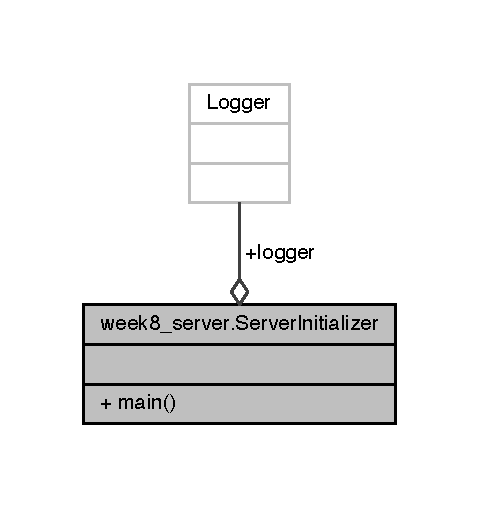
\includegraphics[width=230pt]{classweek8__server_1_1_server_initializer__coll__graph}
\end{center}
\end{figure}
\subsection*{정적 Public 멤버 함수}
\begin{DoxyCompactItemize}
\item 
static void \hyperlink{classweek8__server_1_1_server_initializer_a73b9694a5855a87335cbe63c96f8c8a9}{main} (String\mbox{[}$\,$\mbox{]} args)
\begin{DoxyCompactList}\small\item\em project main method \end{DoxyCompactList}\end{DoxyCompactItemize}
\subsection*{정적 Public 속성}
\begin{DoxyCompactItemize}
\item 
static Logger \hyperlink{classweek8__server_1_1_server_initializer_a93ccaaf656ba68e2dd3950bacc0e9b2e}{logger}
\end{DoxyCompactItemize}


\subsection{상세한 설명}
Initializer class for Reactor-\/\-Thread using server. 

\begin{DoxyDate}{날짜}
2014-\/09-\/17 
\end{DoxyDate}
\begin{DoxyAuthor}{작성자}
youngkim, \href{mailto:ky200223@nhnnext.org}{\tt ky200223@nhnnext.\-org}
\end{DoxyAuthor}
Initialize and start \hyperlink{classweek8__server_1_1_reactor}{Reactor} server on port 5000, using handler\-List.\-xml for dynamic class loading 

Server\-Initializer.\-java 파일의 29 번째 라인에서 정의되었습니다.



\subsection{멤버 함수 문서화}
\hypertarget{classweek8__server_1_1_server_initializer_a73b9694a5855a87335cbe63c96f8c8a9}{\index{week8\-\_\-server\-::\-Server\-Initializer@{week8\-\_\-server\-::\-Server\-Initializer}!main@{main}}
\index{main@{main}!week8_server::ServerInitializer@{week8\-\_\-server\-::\-Server\-Initializer}}
\subsubsection[{main}]{\setlength{\rightskip}{0pt plus 5cm}static void week8\-\_\-server.\-Server\-Initializer.\-main (
\begin{DoxyParamCaption}
\item[{String\mbox{[}$\,$\mbox{]}}]{args}
\end{DoxyParamCaption}
)\hspace{0.3cm}{\ttfamily [static]}}}\label{classweek8__server_1_1_server_initializer_a73b9694a5855a87335cbe63c96f8c8a9}


project main method 

initialize and start reactor server 
\begin{DoxyParams}{매개변수}
{\em none} & \\
\hline
\end{DoxyParams}
\begin{DoxyReturn}{반환값}
none 
\end{DoxyReturn}


Server\-Initializer.\-java 파일의 40 번째 라인에서 정의되었습니다.


\begin{DoxyCode}
40                                            \{
41         \textcolor{keywordtype}{int} port = 5000;
42         System.out.println(\textcolor{stringliteral}{"Server ON : "} + port);
43         logger.info(\textcolor{stringliteral}{"Server ON : "} + port);
44 
45         logger.fatal(\textcolor{stringliteral}{"log4j:logger.fatal()"});
46         logger.error(\textcolor{stringliteral}{"log4j:logger.error()"});
47         logger.warn(\textcolor{stringliteral}{"log4j:logger.warn()"});
48         logger.info(\textcolor{stringliteral}{"log4j:logger.info()"});
49         logger.debug(\textcolor{stringliteral}{"log4j:logger.debug()"});
50         logger.trace(\textcolor{stringliteral}{"log4j:logger.trace()"});
51 
52         Reactor reactor = \textcolor{keyword}{new} Reactor(port);
53 
54         Serializer serializer = \textcolor{keyword}{new} Persister();
55         File source = \textcolor{keyword}{new} File(\textcolor{stringliteral}{"HandlerList.xml"});
56         \textcolor{keywordflow}{try} \{
57             ServerListData serverList = serializer.read(ServerListData.class,
58                     source);
59 
60             \textcolor{keywordflow}{for} (HandlerListData handlerListData : serverList.getServer()) \{
61                 \textcolor{keywordflow}{if} (\textcolor{stringliteral}{"server1"}.equals(handlerListData.getName())) \{
62                     List<String> handlerList = handlerListData.getHandler();
63                     \textcolor{keywordflow}{for} (String handler : handlerList) \{
64                         \textcolor{keywordflow}{try} \{
65                             reactor.registerHandler((EventHandler) Class
66                                     .forName(handler).newInstance());
67                         \} \textcolor{keywordflow}{catch} (InstantiationException e) \{
68                             e.printStackTrace();
69                         \} \textcolor{keywordflow}{catch} (IllegalAccessException e) \{
70                             e.printStackTrace();
71                         \} \textcolor{keywordflow}{catch} (ClassNotFoundException e) \{
72                             e.printStackTrace();
73                         \}
74                     \}
75                 \}
76             \}
77         \} \textcolor{keywordflow}{catch} (Exception e) \{
78             e.printStackTrace();
79         \}
80 
81         reactor.startServer();
82     \}
\end{DoxyCode}


이 함수 내부에서 호출하는 함수들에 대한 그래프입니다.\-:
\nopagebreak
\begin{figure}[H]
\begin{center}
\leavevmode
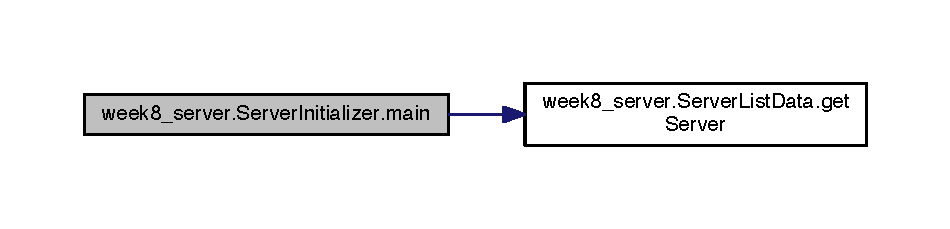
\includegraphics[width=350pt]{classweek8__server_1_1_server_initializer_a73b9694a5855a87335cbe63c96f8c8a9_cgraph}
\end{center}
\end{figure}




\subsection{멤버 데이타 문서화}
\hypertarget{classweek8__server_1_1_server_initializer_a93ccaaf656ba68e2dd3950bacc0e9b2e}{\index{week8\-\_\-server\-::\-Server\-Initializer@{week8\-\_\-server\-::\-Server\-Initializer}!logger@{logger}}
\index{logger@{logger}!week8_server::ServerInitializer@{week8\-\_\-server\-::\-Server\-Initializer}}
\subsubsection[{logger}]{\setlength{\rightskip}{0pt plus 5cm}Logger week8\-\_\-server.\-Server\-Initializer.\-logger\hspace{0.3cm}{\ttfamily [static]}}}\label{classweek8__server_1_1_server_initializer_a93ccaaf656ba68e2dd3950bacc0e9b2e}
{\bfseries 초기값\-:}
\begin{DoxyCode}
= Logger.getLogger(ServerInitializer.class
            .getName())
\end{DoxyCode}


Server\-Initializer.\-java 파일의 31 번째 라인에서 정의되었습니다.



이 클래스에 대한 문서화 페이지는 다음의 파일로부터 생성되었습니다.\-:\begin{DoxyCompactItemize}
\item 
src/week8\-\_\-server/\hyperlink{_server_initializer_8java}{Server\-Initializer.\-java}\end{DoxyCompactItemize}

\hypertarget{classweek8__server_1_1_server_list_data}{\section{week8\-\_\-server.\-Server\-List\-Data 클래스 참조}
\label{classweek8__server_1_1_server_list_data}\index{week8\-\_\-server.\-Server\-List\-Data@{week8\-\_\-server.\-Server\-List\-Data}}
}


week8\-\_\-server.\-Server\-List\-Data에 대한 협력 다이어그램\-:
\nopagebreak
\begin{figure}[H]
\begin{center}
\leavevmode
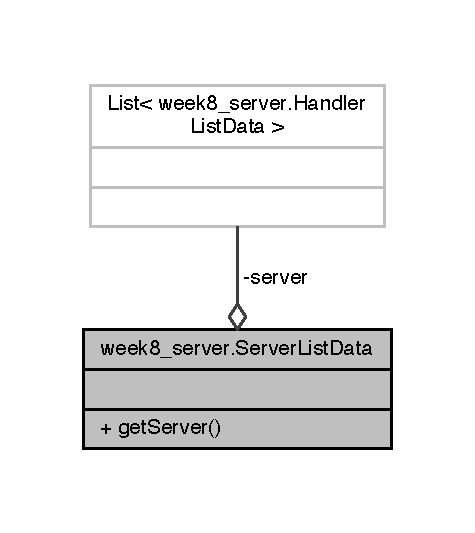
\includegraphics[width=228pt]{classweek8__server_1_1_server_list_data__coll__graph}
\end{center}
\end{figure}
\subsection*{Public 멤버 함수}
\begin{DoxyCompactItemize}
\item 
List$<$ \hyperlink{classweek8__server_1_1_handler_list_data}{Handler\-List\-Data} $>$ \hyperlink{classweek8__server_1_1_server_list_data_a290deb1c104276fd65c014e4e4d790f0}{get\-Server} ()
\end{DoxyCompactItemize}
\subsection*{Private 속성}
\begin{DoxyCompactItemize}
\item 
List$<$ \hyperlink{classweek8__server_1_1_handler_list_data}{Handler\-List\-Data} $>$ \hyperlink{classweek8__server_1_1_server_list_data_a732d8343a7bb9f2afd473a397a9937aa}{server}
\end{DoxyCompactItemize}


\subsection{상세한 설명}


Server\-List\-Data.\-java 파일의 19 번째 라인에서 정의되었습니다.



\subsection{멤버 함수 문서화}
\hypertarget{classweek8__server_1_1_server_list_data_a290deb1c104276fd65c014e4e4d790f0}{\index{week8\-\_\-server\-::\-Server\-List\-Data@{week8\-\_\-server\-::\-Server\-List\-Data}!get\-Server@{get\-Server}}
\index{get\-Server@{get\-Server}!week8_server::ServerListData@{week8\-\_\-server\-::\-Server\-List\-Data}}
\subsubsection[{get\-Server}]{\setlength{\rightskip}{0pt plus 5cm}List$<${\bf Handler\-List\-Data}$>$ week8\-\_\-server.\-Server\-List\-Data.\-get\-Server (
\begin{DoxyParamCaption}
{}
\end{DoxyParamCaption}
)}}\label{classweek8__server_1_1_server_list_data_a290deb1c104276fd65c014e4e4d790f0}


Server\-List\-Data.\-java 파일의 23 번째 라인에서 정의되었습니다.


\begin{DoxyCode}
23                                              \{
24         \textcolor{keywordflow}{return} \hyperlink{classweek8__server_1_1_server_list_data_a732d8343a7bb9f2afd473a397a9937aa}{server};
25     \}
\end{DoxyCode}


이 함수를 호출하는 함수들에 대한 그래프입니다.\-:
\nopagebreak
\begin{figure}[H]
\begin{center}
\leavevmode
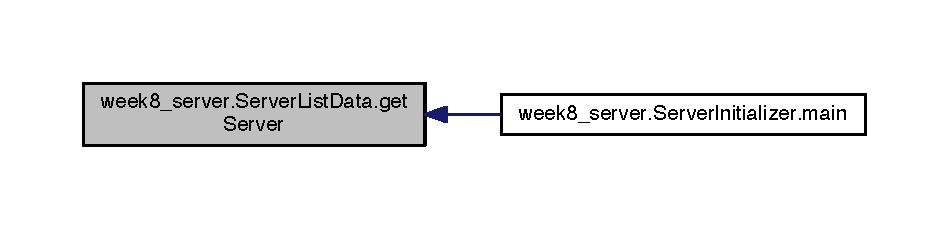
\includegraphics[width=350pt]{classweek8__server_1_1_server_list_data_a290deb1c104276fd65c014e4e4d790f0_icgraph}
\end{center}
\end{figure}




\subsection{멤버 데이타 문서화}
\hypertarget{classweek8__server_1_1_server_list_data_a732d8343a7bb9f2afd473a397a9937aa}{\index{week8\-\_\-server\-::\-Server\-List\-Data@{week8\-\_\-server\-::\-Server\-List\-Data}!server@{server}}
\index{server@{server}!week8_server::ServerListData@{week8\-\_\-server\-::\-Server\-List\-Data}}
\subsubsection[{server}]{\setlength{\rightskip}{0pt plus 5cm}List$<${\bf Handler\-List\-Data}$>$ week8\-\_\-server.\-Server\-List\-Data.\-server\hspace{0.3cm}{\ttfamily [private]}}}\label{classweek8__server_1_1_server_list_data_a732d8343a7bb9f2afd473a397a9937aa}


Server\-List\-Data.\-java 파일의 21 번째 라인에서 정의되었습니다.



이 클래스에 대한 문서화 페이지는 다음의 파일로부터 생성되었습니다.\-:\begin{DoxyCompactItemize}
\item 
src/week8\-\_\-server/\hyperlink{_server_list_data_8java}{Server\-List\-Data.\-java}\end{DoxyCompactItemize}

\hypertarget{classweek8__server_1_1_stream_say_hello_event_handler}{\section{week8\-\_\-server.\-Stream\-Say\-Hello\-Event\-Handler 클래스 참조}
\label{classweek8__server_1_1_stream_say_hello_event_handler}\index{week8\-\_\-server.\-Stream\-Say\-Hello\-Event\-Handler@{week8\-\_\-server.\-Stream\-Say\-Hello\-Event\-Handler}}
}


route request with header info to each handler  




week8\-\_\-server.\-Stream\-Say\-Hello\-Event\-Handler에 대한 상속 다이어그램 \-: 
\nopagebreak
\begin{figure}[H]
\begin{center}
\leavevmode
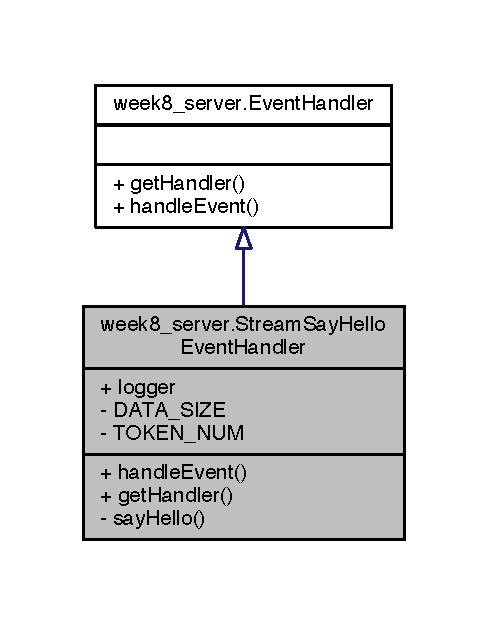
\includegraphics[width=234pt]{classweek8__server_1_1_stream_say_hello_event_handler__inherit__graph}
\end{center}
\end{figure}


week8\-\_\-server.\-Stream\-Say\-Hello\-Event\-Handler에 대한 협력 다이어그램\-:
\nopagebreak
\begin{figure}[H]
\begin{center}
\leavevmode
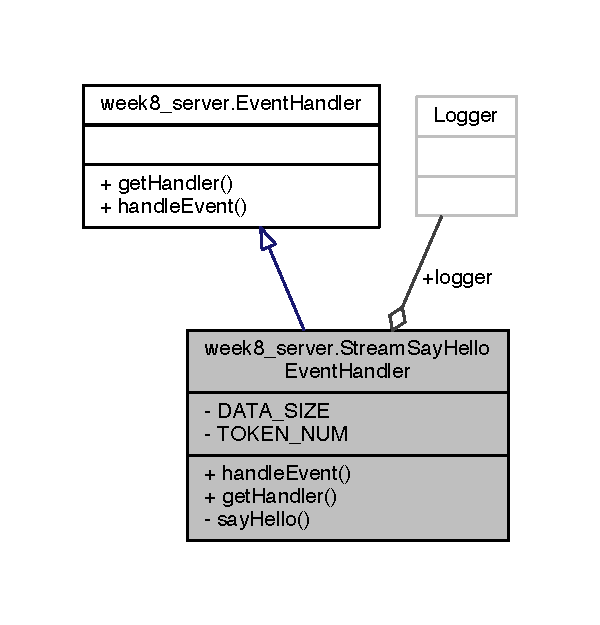
\includegraphics[width=288pt]{classweek8__server_1_1_stream_say_hello_event_handler__coll__graph}
\end{center}
\end{figure}
\subsection*{Public 멤버 함수}
\begin{DoxyCompactItemize}
\item 
void \hyperlink{classweek8__server_1_1_stream_say_hello_event_handler_a2c2be02c3987ca818d6c09fd800d0f34}{handle\-Event} (Input\-Stream is)
\begin{DoxyCompactList}\small\item\em request handler \end{DoxyCompactList}\item 
String \hyperlink{classweek8__server_1_1_stream_say_hello_event_handler_a179e9b7dae2e32891de7dbc707e3d07e}{get\-Handler} ()
\end{DoxyCompactItemize}
\subsection*{정적 Public 속성}
\begin{DoxyCompactItemize}
\item 
static Logger \hyperlink{classweek8__server_1_1_stream_say_hello_event_handler_a68c45171ab9184973fa32d5b18f1fc70}{logger}
\end{DoxyCompactItemize}
\subsection*{Private 멤버 함수}
\begin{DoxyCompactItemize}
\item 
void \hyperlink{classweek8__server_1_1_stream_say_hello_event_handler_ad250ce0474a5ef1f7820ac2f03bac221}{say\-Hello} (String\mbox{[}$\,$\mbox{]} params)
\begin{DoxyCompactList}\small\item\em print request \end{DoxyCompactList}\end{DoxyCompactItemize}
\subsection*{정적 Private 속성}
\begin{DoxyCompactItemize}
\item 
static final int \hyperlink{classweek8__server_1_1_stream_say_hello_event_handler_aaaadade47c5c1093fa1b82e876039036}{D\-A\-T\-A\-\_\-\-S\-I\-Z\-E} = 512
\item 
static final int \hyperlink{classweek8__server_1_1_stream_say_hello_event_handler_aa6b191144a3deebb3779ddad8a10850d}{T\-O\-K\-E\-N\-\_\-\-N\-U\-M} = 2
\end{DoxyCompactItemize}


\subsection{상세한 설명}
route request with header info to each handler 

\begin{DoxyDate}{날짜}
2014-\/09-\/17 
\end{DoxyDate}
\begin{DoxyAuthor}{작성자}
youngkim, \href{mailto:ky200223@nhnnext.org}{\tt ky200223@nhnnext.\-org}
\end{DoxyAuthor}
get request that start with 0x5001(header) and print result 

Stream\-Say\-Hello\-Event\-Handler.\-java 파일의 26 번째 라인에서 정의되었습니다.



\subsection{멤버 함수 문서화}
\hypertarget{classweek8__server_1_1_stream_say_hello_event_handler_a179e9b7dae2e32891de7dbc707e3d07e}{\index{week8\-\_\-server\-::\-Stream\-Say\-Hello\-Event\-Handler@{week8\-\_\-server\-::\-Stream\-Say\-Hello\-Event\-Handler}!get\-Handler@{get\-Handler}}
\index{get\-Handler@{get\-Handler}!week8_server::StreamSayHelloEventHandler@{week8\-\_\-server\-::\-Stream\-Say\-Hello\-Event\-Handler}}
\subsubsection[{get\-Handler}]{\setlength{\rightskip}{0pt plus 5cm}String week8\-\_\-server.\-Stream\-Say\-Hello\-Event\-Handler.\-get\-Handler (
\begin{DoxyParamCaption}
{}
\end{DoxyParamCaption}
)}}\label{classweek8__server_1_1_stream_say_hello_event_handler_a179e9b7dae2e32891de7dbc707e3d07e}


\hyperlink{interfaceweek8__server_1_1_event_handler_a77b9a43471e25538de361dd0fff9478b}{week8\-\_\-server.\-Event\-Handler}를 구현.



Stream\-Say\-Hello\-Event\-Handler.\-java 파일의 75 번째 라인에서 정의되었습니다.


\begin{DoxyCode}
75                                \{
76         \textcolor{keywordflow}{return} \textcolor{stringliteral}{"0x5001"};
77     \}
\end{DoxyCode}
\hypertarget{classweek8__server_1_1_stream_say_hello_event_handler_a2c2be02c3987ca818d6c09fd800d0f34}{\index{week8\-\_\-server\-::\-Stream\-Say\-Hello\-Event\-Handler@{week8\-\_\-server\-::\-Stream\-Say\-Hello\-Event\-Handler}!handle\-Event@{handle\-Event}}
\index{handle\-Event@{handle\-Event}!week8_server::StreamSayHelloEventHandler@{week8\-\_\-server\-::\-Stream\-Say\-Hello\-Event\-Handler}}
\subsubsection[{handle\-Event}]{\setlength{\rightskip}{0pt plus 5cm}void week8\-\_\-server.\-Stream\-Say\-Hello\-Event\-Handler.\-handle\-Event (
\begin{DoxyParamCaption}
\item[{Input\-Stream}]{is}
\end{DoxyParamCaption}
)}}\label{classweek8__server_1_1_stream_say_hello_event_handler_a2c2be02c3987ca818d6c09fd800d0f34}


request handler 

read stream and tokenize for get each data 
\begin{DoxyParams}{매개변수}
{\em is} & (inputstream) \\
\hline
\end{DoxyParams}
\begin{DoxyReturn}{반환값}
none 
\end{DoxyReturn}


\hyperlink{interfaceweek8__server_1_1_event_handler_a24d2832c020ae27428c12be6d5277e51}{week8\-\_\-server.\-Event\-Handler}를 구현.



Stream\-Say\-Hello\-Event\-Handler.\-java 파일의 40 번째 라인에서 정의되었습니다.


\begin{DoxyCode}
40                                             \{
41 
42         \textcolor{keywordflow}{try} \{
43             byte[] buffer = \textcolor{keyword}{new} byte[\hyperlink{classweek8__server_1_1_stream_say_hello_event_handler_aaaadade47c5c1093fa1b82e876039036}{DATA\_SIZE}];
44             is.read(buffer);
45             String data = \textcolor{keyword}{new} String(buffer);
46 
47             String[] params = \textcolor{keyword}{new} String[\hyperlink{classweek8__server_1_1_stream_say_hello_event_handler_aa6b191144a3deebb3779ddad8a10850d}{TOKEN\_NUM}];
48             StringTokenizer token = \textcolor{keyword}{new} StringTokenizer(data, \textcolor{stringliteral}{"|"});
49 
50             \textcolor{keywordtype}{int} i = 0;
51             \textcolor{keywordflow}{while} (token.hasMoreTokens()) \{
52                 params[i] = token.nextToken();
53                 ++i;
54             \}
55 
56             \hyperlink{classweek8__server_1_1_stream_say_hello_event_handler_ad250ce0474a5ef1f7820ac2f03bac221}{sayHello}(params);
57 
58         \} \textcolor{keywordflow}{catch} (IOException e) \{
59             e.printStackTrace();
60         \}
61     \}
\end{DoxyCode}


이 함수 내부에서 호출하는 함수들에 대한 그래프입니다.\-:
\nopagebreak
\begin{figure}[H]
\begin{center}
\leavevmode
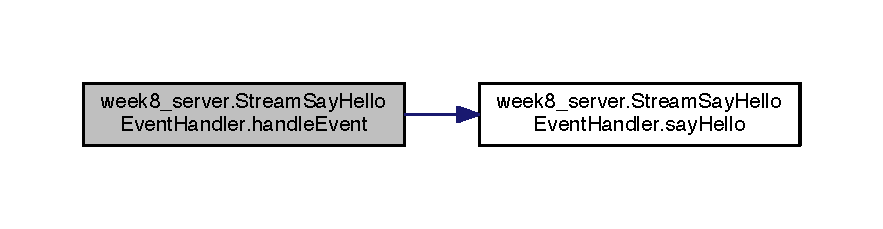
\includegraphics[width=350pt]{classweek8__server_1_1_stream_say_hello_event_handler_a2c2be02c3987ca818d6c09fd800d0f34_cgraph}
\end{center}
\end{figure}


\hypertarget{classweek8__server_1_1_stream_say_hello_event_handler_ad250ce0474a5ef1f7820ac2f03bac221}{\index{week8\-\_\-server\-::\-Stream\-Say\-Hello\-Event\-Handler@{week8\-\_\-server\-::\-Stream\-Say\-Hello\-Event\-Handler}!say\-Hello@{say\-Hello}}
\index{say\-Hello@{say\-Hello}!week8_server::StreamSayHelloEventHandler@{week8\-\_\-server\-::\-Stream\-Say\-Hello\-Event\-Handler}}
\subsubsection[{say\-Hello}]{\setlength{\rightskip}{0pt plus 5cm}void week8\-\_\-server.\-Stream\-Say\-Hello\-Event\-Handler.\-say\-Hello (
\begin{DoxyParamCaption}
\item[{String\mbox{[}$\,$\mbox{]}}]{params}
\end{DoxyParamCaption}
)\hspace{0.3cm}{\ttfamily [private]}}}\label{classweek8__server_1_1_stream_say_hello_event_handler_ad250ce0474a5ef1f7820ac2f03bac221}


print request 


\begin{DoxyParams}{매개변수}
{\em string\mbox{[}$\,$\mbox{]}} & \\
\hline
\end{DoxyParams}
\begin{DoxyReturn}{반환값}
none 
\end{DoxyReturn}


Stream\-Say\-Hello\-Event\-Handler.\-java 파일의 68 번째 라인에서 정의되었습니다.


\begin{DoxyCode}
68                                            \{
69         System.out.println(\textcolor{stringliteral}{"SayHello -> name : "} + params[0] + \textcolor{stringliteral}{"age : "}
70                 + params[1]);
71         logger.info(\textcolor{stringliteral}{"SayHello -> name : "} + params[0] + \textcolor{stringliteral}{"age : "} + params[1]);
72     \}
\end{DoxyCode}


이 함수를 호출하는 함수들에 대한 그래프입니다.\-:
\nopagebreak
\begin{figure}[H]
\begin{center}
\leavevmode
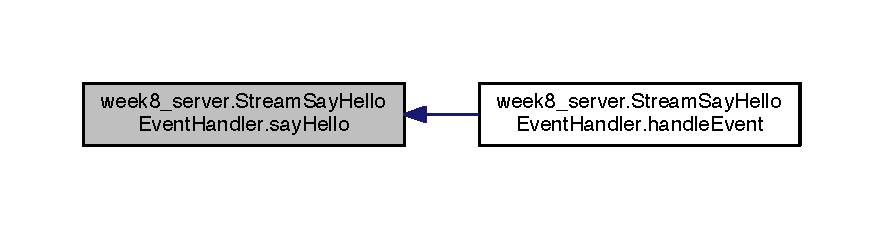
\includegraphics[width=350pt]{classweek8__server_1_1_stream_say_hello_event_handler_ad250ce0474a5ef1f7820ac2f03bac221_icgraph}
\end{center}
\end{figure}




\subsection{멤버 데이타 문서화}
\hypertarget{classweek8__server_1_1_stream_say_hello_event_handler_aaaadade47c5c1093fa1b82e876039036}{\index{week8\-\_\-server\-::\-Stream\-Say\-Hello\-Event\-Handler@{week8\-\_\-server\-::\-Stream\-Say\-Hello\-Event\-Handler}!D\-A\-T\-A\-\_\-\-S\-I\-Z\-E@{D\-A\-T\-A\-\_\-\-S\-I\-Z\-E}}
\index{D\-A\-T\-A\-\_\-\-S\-I\-Z\-E@{D\-A\-T\-A\-\_\-\-S\-I\-Z\-E}!week8_server::StreamSayHelloEventHandler@{week8\-\_\-server\-::\-Stream\-Say\-Hello\-Event\-Handler}}
\subsubsection[{D\-A\-T\-A\-\_\-\-S\-I\-Z\-E}]{\setlength{\rightskip}{0pt plus 5cm}final int week8\-\_\-server.\-Stream\-Say\-Hello\-Event\-Handler.\-D\-A\-T\-A\-\_\-\-S\-I\-Z\-E = 512\hspace{0.3cm}{\ttfamily [static]}, {\ttfamily [private]}}}\label{classweek8__server_1_1_stream_say_hello_event_handler_aaaadade47c5c1093fa1b82e876039036}


Stream\-Say\-Hello\-Event\-Handler.\-java 파일의 31 번째 라인에서 정의되었습니다.

\hypertarget{classweek8__server_1_1_stream_say_hello_event_handler_a68c45171ab9184973fa32d5b18f1fc70}{\index{week8\-\_\-server\-::\-Stream\-Say\-Hello\-Event\-Handler@{week8\-\_\-server\-::\-Stream\-Say\-Hello\-Event\-Handler}!logger@{logger}}
\index{logger@{logger}!week8_server::StreamSayHelloEventHandler@{week8\-\_\-server\-::\-Stream\-Say\-Hello\-Event\-Handler}}
\subsubsection[{logger}]{\setlength{\rightskip}{0pt plus 5cm}Logger week8\-\_\-server.\-Stream\-Say\-Hello\-Event\-Handler.\-logger\hspace{0.3cm}{\ttfamily [static]}}}\label{classweek8__server_1_1_stream_say_hello_event_handler_a68c45171ab9184973fa32d5b18f1fc70}
{\bfseries 초기값\-:}
\begin{DoxyCode}
= Logger.getLogger(ServerInitializer.class
            .getName())
\end{DoxyCode}


Stream\-Say\-Hello\-Event\-Handler.\-java 파일의 28 번째 라인에서 정의되었습니다.

\hypertarget{classweek8__server_1_1_stream_say_hello_event_handler_aa6b191144a3deebb3779ddad8a10850d}{\index{week8\-\_\-server\-::\-Stream\-Say\-Hello\-Event\-Handler@{week8\-\_\-server\-::\-Stream\-Say\-Hello\-Event\-Handler}!T\-O\-K\-E\-N\-\_\-\-N\-U\-M@{T\-O\-K\-E\-N\-\_\-\-N\-U\-M}}
\index{T\-O\-K\-E\-N\-\_\-\-N\-U\-M@{T\-O\-K\-E\-N\-\_\-\-N\-U\-M}!week8_server::StreamSayHelloEventHandler@{week8\-\_\-server\-::\-Stream\-Say\-Hello\-Event\-Handler}}
\subsubsection[{T\-O\-K\-E\-N\-\_\-\-N\-U\-M}]{\setlength{\rightskip}{0pt plus 5cm}final int week8\-\_\-server.\-Stream\-Say\-Hello\-Event\-Handler.\-T\-O\-K\-E\-N\-\_\-\-N\-U\-M = 2\hspace{0.3cm}{\ttfamily [static]}, {\ttfamily [private]}}}\label{classweek8__server_1_1_stream_say_hello_event_handler_aa6b191144a3deebb3779ddad8a10850d}


Stream\-Say\-Hello\-Event\-Handler.\-java 파일의 32 번째 라인에서 정의되었습니다.



이 클래스에 대한 문서화 페이지는 다음의 파일로부터 생성되었습니다.\-:\begin{DoxyCompactItemize}
\item 
src/week8\-\_\-server/\hyperlink{_stream_say_hello_event_handler_8java}{Stream\-Say\-Hello\-Event\-Handler.\-java}\end{DoxyCompactItemize}

\hypertarget{classweek8__server_1_1_stream_update_profile_event_handler}{\section{week8\-\_\-server.\-Stream\-Update\-Profile\-Event\-Handler 클래스 참조}
\label{classweek8__server_1_1_stream_update_profile_event_handler}\index{week8\-\_\-server.\-Stream\-Update\-Profile\-Event\-Handler@{week8\-\_\-server.\-Stream\-Update\-Profile\-Event\-Handler}}
}


route request with header info to each handler  




week8\-\_\-server.\-Stream\-Update\-Profile\-Event\-Handler에 대한 상속 다이어그램 \-: 
\nopagebreak
\begin{figure}[H]
\begin{center}
\leavevmode
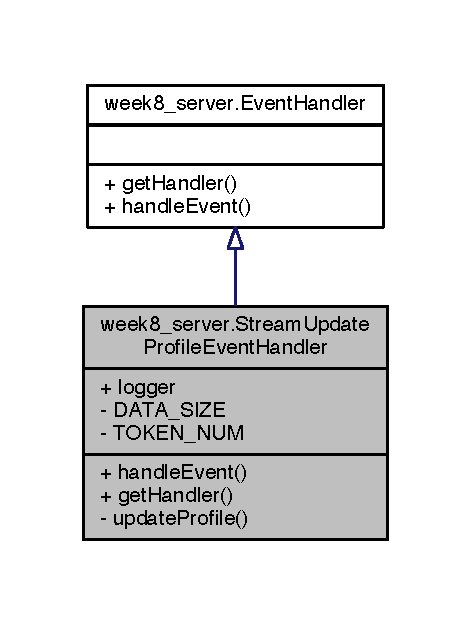
\includegraphics[width=226pt]{classweek8__server_1_1_stream_update_profile_event_handler__inherit__graph}
\end{center}
\end{figure}


week8\-\_\-server.\-Stream\-Update\-Profile\-Event\-Handler에 대한 협력 다이어그램\-:
\nopagebreak
\begin{figure}[H]
\begin{center}
\leavevmode
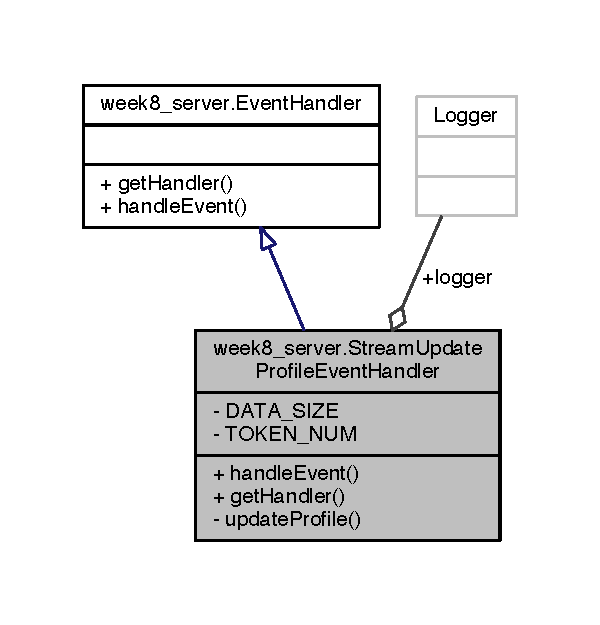
\includegraphics[width=288pt]{classweek8__server_1_1_stream_update_profile_event_handler__coll__graph}
\end{center}
\end{figure}
\subsection*{Public 멤버 함수}
\begin{DoxyCompactItemize}
\item 
void \hyperlink{classweek8__server_1_1_stream_update_profile_event_handler_a9cf985ef61eff5226bc397d72847abed}{handle\-Event} (Input\-Stream is)
\begin{DoxyCompactList}\small\item\em request handler \end{DoxyCompactList}\item 
String \hyperlink{classweek8__server_1_1_stream_update_profile_event_handler_a0f5b195408dd8fb6b250ce8531a71f02}{get\-Handler} ()
\end{DoxyCompactItemize}
\subsection*{정적 Public 속성}
\begin{DoxyCompactItemize}
\item 
static Logger \hyperlink{classweek8__server_1_1_stream_update_profile_event_handler_ad704bc0908f0f6b43b7cc21887990f0e}{logger}
\end{DoxyCompactItemize}
\subsection*{Private 멤버 함수}
\begin{DoxyCompactItemize}
\item 
void \hyperlink{classweek8__server_1_1_stream_update_profile_event_handler_ab2a9e69d8c970f9f8ea254337f53f558}{update\-Profile} (String\mbox{[}$\,$\mbox{]} params)
\begin{DoxyCompactList}\small\item\em print request \end{DoxyCompactList}\end{DoxyCompactItemize}
\subsection*{정적 Private 속성}
\begin{DoxyCompactItemize}
\item 
static final int \hyperlink{classweek8__server_1_1_stream_update_profile_event_handler_aa635f419e6b73e10089f152538ce0b51}{D\-A\-T\-A\-\_\-\-S\-I\-Z\-E} = 1024
\item 
static final int \hyperlink{classweek8__server_1_1_stream_update_profile_event_handler_a23249215f663a5224287bb8e0c9d0588}{T\-O\-K\-E\-N\-\_\-\-N\-U\-M} = 5
\end{DoxyCompactItemize}


\subsection{상세한 설명}
route request with header info to each handler 

\begin{DoxyDate}{날짜}
2014-\/09-\/17 
\end{DoxyDate}
\begin{DoxyAuthor}{작성자}
youngkim, \href{mailto:ky200223@nhnnext.org}{\tt ky200223@nhnnext.\-org}
\end{DoxyAuthor}
get request that start with 0x6001(header) and print result 

Stream\-Update\-Profile\-Event\-Handler.\-java 파일의 26 번째 라인에서 정의되었습니다.



\subsection{멤버 함수 문서화}
\hypertarget{classweek8__server_1_1_stream_update_profile_event_handler_a0f5b195408dd8fb6b250ce8531a71f02}{\index{week8\-\_\-server\-::\-Stream\-Update\-Profile\-Event\-Handler@{week8\-\_\-server\-::\-Stream\-Update\-Profile\-Event\-Handler}!get\-Handler@{get\-Handler}}
\index{get\-Handler@{get\-Handler}!week8_server::StreamUpdateProfileEventHandler@{week8\-\_\-server\-::\-Stream\-Update\-Profile\-Event\-Handler}}
\subsubsection[{get\-Handler}]{\setlength{\rightskip}{0pt plus 5cm}String week8\-\_\-server.\-Stream\-Update\-Profile\-Event\-Handler.\-get\-Handler (
\begin{DoxyParamCaption}
{}
\end{DoxyParamCaption}
)}}\label{classweek8__server_1_1_stream_update_profile_event_handler_a0f5b195408dd8fb6b250ce8531a71f02}


\hyperlink{interfaceweek8__server_1_1_event_handler_a77b9a43471e25538de361dd0fff9478b}{week8\-\_\-server.\-Event\-Handler}를 구현.



Stream\-Update\-Profile\-Event\-Handler.\-java 파일의 75 번째 라인에서 정의되었습니다.


\begin{DoxyCode}
75                                \{
76         \textcolor{keywordflow}{return} \textcolor{stringliteral}{"0x6001"};
77     \}
\end{DoxyCode}
\hypertarget{classweek8__server_1_1_stream_update_profile_event_handler_a9cf985ef61eff5226bc397d72847abed}{\index{week8\-\_\-server\-::\-Stream\-Update\-Profile\-Event\-Handler@{week8\-\_\-server\-::\-Stream\-Update\-Profile\-Event\-Handler}!handle\-Event@{handle\-Event}}
\index{handle\-Event@{handle\-Event}!week8_server::StreamUpdateProfileEventHandler@{week8\-\_\-server\-::\-Stream\-Update\-Profile\-Event\-Handler}}
\subsubsection[{handle\-Event}]{\setlength{\rightskip}{0pt plus 5cm}void week8\-\_\-server.\-Stream\-Update\-Profile\-Event\-Handler.\-handle\-Event (
\begin{DoxyParamCaption}
\item[{Input\-Stream}]{is}
\end{DoxyParamCaption}
)}}\label{classweek8__server_1_1_stream_update_profile_event_handler_a9cf985ef61eff5226bc397d72847abed}


request handler 

read stream and tokenize for get each data 
\begin{DoxyParams}{매개변수}
{\em is} & (inputstream) \\
\hline
\end{DoxyParams}
\begin{DoxyReturn}{반환값}
none 
\end{DoxyReturn}


\hyperlink{interfaceweek8__server_1_1_event_handler_a24d2832c020ae27428c12be6d5277e51}{week8\-\_\-server.\-Event\-Handler}를 구현.



Stream\-Update\-Profile\-Event\-Handler.\-java 파일의 40 번째 라인에서 정의되었습니다.


\begin{DoxyCode}
40                                             \{
41 
42         \textcolor{keywordflow}{try} \{
43             byte[] buffer = \textcolor{keyword}{new} byte[\hyperlink{classweek8__server_1_1_stream_update_profile_event_handler_aa635f419e6b73e10089f152538ce0b51}{DATA\_SIZE}];
44             is.read(buffer);
45             String data = \textcolor{keyword}{new} String(buffer);
46 
47             String[] params = \textcolor{keyword}{new} String[\hyperlink{classweek8__server_1_1_stream_update_profile_event_handler_a23249215f663a5224287bb8e0c9d0588}{TOKEN\_NUM}];
48             StringTokenizer token = \textcolor{keyword}{new} StringTokenizer(data, \textcolor{stringliteral}{"|"});
49 
50             \textcolor{keywordtype}{int} i = 0;
51             \textcolor{keywordflow}{while} (token.hasMoreTokens()) \{
52                 params[i] = token.nextToken();
53                 ++i;
54             \}
55 
56             \hyperlink{classweek8__server_1_1_stream_update_profile_event_handler_ab2a9e69d8c970f9f8ea254337f53f558}{updateProfile}(params);
57 
58         \} \textcolor{keywordflow}{catch} (IOException e) \{
59             e.printStackTrace();
60         \}
61     \}
\end{DoxyCode}


이 함수 내부에서 호출하는 함수들에 대한 그래프입니다.\-:
\nopagebreak
\begin{figure}[H]
\begin{center}
\leavevmode
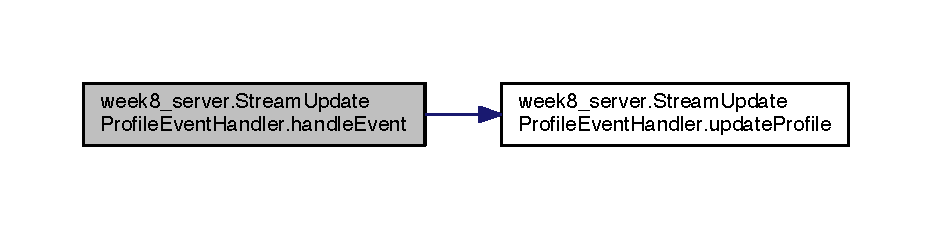
\includegraphics[width=350pt]{classweek8__server_1_1_stream_update_profile_event_handler_a9cf985ef61eff5226bc397d72847abed_cgraph}
\end{center}
\end{figure}


\hypertarget{classweek8__server_1_1_stream_update_profile_event_handler_ab2a9e69d8c970f9f8ea254337f53f558}{\index{week8\-\_\-server\-::\-Stream\-Update\-Profile\-Event\-Handler@{week8\-\_\-server\-::\-Stream\-Update\-Profile\-Event\-Handler}!update\-Profile@{update\-Profile}}
\index{update\-Profile@{update\-Profile}!week8_server::StreamUpdateProfileEventHandler@{week8\-\_\-server\-::\-Stream\-Update\-Profile\-Event\-Handler}}
\subsubsection[{update\-Profile}]{\setlength{\rightskip}{0pt plus 5cm}void week8\-\_\-server.\-Stream\-Update\-Profile\-Event\-Handler.\-update\-Profile (
\begin{DoxyParamCaption}
\item[{String\mbox{[}$\,$\mbox{]}}]{params}
\end{DoxyParamCaption}
)\hspace{0.3cm}{\ttfamily [private]}}}\label{classweek8__server_1_1_stream_update_profile_event_handler_ab2a9e69d8c970f9f8ea254337f53f558}


print request 


\begin{DoxyParams}{매개변수}
{\em string\mbox{[}$\,$\mbox{]}} & \\
\hline
\end{DoxyParams}
\begin{DoxyReturn}{반환값}
none 
\end{DoxyReturn}


Stream\-Update\-Profile\-Event\-Handler.\-java 파일의 68 번째 라인에서 정의되었습니다.


\begin{DoxyCode}
68                                                 \{
69         logger.info(\textcolor{stringliteral}{"UpdateProfile -> "} + \textcolor{stringliteral}{" id : "} + params[0] + \textcolor{stringliteral}{" password : "}
70                 + params[1] + \textcolor{stringliteral}{" name : "} + params[2] + \textcolor{stringliteral}{" age : "} + params[3]
71                 + \textcolor{stringliteral}{" gender : "} + params[4]);
72     \}
\end{DoxyCode}


이 함수를 호출하는 함수들에 대한 그래프입니다.\-:
\nopagebreak
\begin{figure}[H]
\begin{center}
\leavevmode
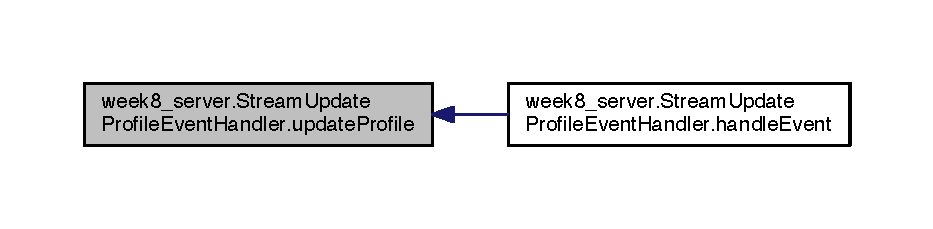
\includegraphics[width=350pt]{classweek8__server_1_1_stream_update_profile_event_handler_ab2a9e69d8c970f9f8ea254337f53f558_icgraph}
\end{center}
\end{figure}




\subsection{멤버 데이타 문서화}
\hypertarget{classweek8__server_1_1_stream_update_profile_event_handler_aa635f419e6b73e10089f152538ce0b51}{\index{week8\-\_\-server\-::\-Stream\-Update\-Profile\-Event\-Handler@{week8\-\_\-server\-::\-Stream\-Update\-Profile\-Event\-Handler}!D\-A\-T\-A\-\_\-\-S\-I\-Z\-E@{D\-A\-T\-A\-\_\-\-S\-I\-Z\-E}}
\index{D\-A\-T\-A\-\_\-\-S\-I\-Z\-E@{D\-A\-T\-A\-\_\-\-S\-I\-Z\-E}!week8_server::StreamUpdateProfileEventHandler@{week8\-\_\-server\-::\-Stream\-Update\-Profile\-Event\-Handler}}
\subsubsection[{D\-A\-T\-A\-\_\-\-S\-I\-Z\-E}]{\setlength{\rightskip}{0pt plus 5cm}final int week8\-\_\-server.\-Stream\-Update\-Profile\-Event\-Handler.\-D\-A\-T\-A\-\_\-\-S\-I\-Z\-E = 1024\hspace{0.3cm}{\ttfamily [static]}, {\ttfamily [private]}}}\label{classweek8__server_1_1_stream_update_profile_event_handler_aa635f419e6b73e10089f152538ce0b51}


Stream\-Update\-Profile\-Event\-Handler.\-java 파일의 31 번째 라인에서 정의되었습니다.

\hypertarget{classweek8__server_1_1_stream_update_profile_event_handler_ad704bc0908f0f6b43b7cc21887990f0e}{\index{week8\-\_\-server\-::\-Stream\-Update\-Profile\-Event\-Handler@{week8\-\_\-server\-::\-Stream\-Update\-Profile\-Event\-Handler}!logger@{logger}}
\index{logger@{logger}!week8_server::StreamUpdateProfileEventHandler@{week8\-\_\-server\-::\-Stream\-Update\-Profile\-Event\-Handler}}
\subsubsection[{logger}]{\setlength{\rightskip}{0pt plus 5cm}Logger week8\-\_\-server.\-Stream\-Update\-Profile\-Event\-Handler.\-logger\hspace{0.3cm}{\ttfamily [static]}}}\label{classweek8__server_1_1_stream_update_profile_event_handler_ad704bc0908f0f6b43b7cc21887990f0e}
{\bfseries 초기값\-:}
\begin{DoxyCode}
= Logger.getLogger(ServerInitializer.class
            .getName())
\end{DoxyCode}


Stream\-Update\-Profile\-Event\-Handler.\-java 파일의 28 번째 라인에서 정의되었습니다.

\hypertarget{classweek8__server_1_1_stream_update_profile_event_handler_a23249215f663a5224287bb8e0c9d0588}{\index{week8\-\_\-server\-::\-Stream\-Update\-Profile\-Event\-Handler@{week8\-\_\-server\-::\-Stream\-Update\-Profile\-Event\-Handler}!T\-O\-K\-E\-N\-\_\-\-N\-U\-M@{T\-O\-K\-E\-N\-\_\-\-N\-U\-M}}
\index{T\-O\-K\-E\-N\-\_\-\-N\-U\-M@{T\-O\-K\-E\-N\-\_\-\-N\-U\-M}!week8_server::StreamUpdateProfileEventHandler@{week8\-\_\-server\-::\-Stream\-Update\-Profile\-Event\-Handler}}
\subsubsection[{T\-O\-K\-E\-N\-\_\-\-N\-U\-M}]{\setlength{\rightskip}{0pt plus 5cm}final int week8\-\_\-server.\-Stream\-Update\-Profile\-Event\-Handler.\-T\-O\-K\-E\-N\-\_\-\-N\-U\-M = 5\hspace{0.3cm}{\ttfamily [static]}, {\ttfamily [private]}}}\label{classweek8__server_1_1_stream_update_profile_event_handler_a23249215f663a5224287bb8e0c9d0588}


Stream\-Update\-Profile\-Event\-Handler.\-java 파일의 32 번째 라인에서 정의되었습니다.



이 클래스에 대한 문서화 페이지는 다음의 파일로부터 생성되었습니다.\-:\begin{DoxyCompactItemize}
\item 
src/week8\-\_\-server/\hyperlink{_stream_update_profile_event_handler_8java}{Stream\-Update\-Profile\-Event\-Handler.\-java}\end{DoxyCompactItemize}

\hypertarget{classweek8__server_1_1_test_client}{\section{week8\-\_\-server.\-Test\-Client 클래스 참조}
\label{classweek8__server_1_1_test_client}\index{week8\-\_\-server.\-Test\-Client@{week8\-\_\-server.\-Test\-Client}}
}


outputstream data for test  




week8\-\_\-server.\-Test\-Client에 대한 협력 다이어그램\-:
\nopagebreak
\begin{figure}[H]
\begin{center}
\leavevmode
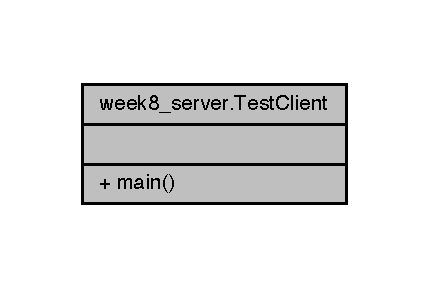
\includegraphics[width=206pt]{classweek8__server_1_1_test_client__coll__graph}
\end{center}
\end{figure}
\subsection*{정적 Public 멤버 함수}
\begin{DoxyCompactItemize}
\item 
static void \hyperlink{classweek8__server_1_1_test_client_aacba0a9c55b57e6805aee049047f5d99}{main} (String\mbox{[}$\,$\mbox{]} args)
\end{DoxyCompactItemize}


\subsection{상세한 설명}
outputstream data for test 

\begin{DoxyDate}{날짜}
2014-\/09-\/17 
\end{DoxyDate}
\begin{DoxyAuthor}{작성자}
youngkim, \href{mailto:ky200223@nhnnext.org}{\tt ky200223@nhnnext.\-org}
\end{DoxyAuthor}
outputstream date for test (2type -\/ different\-Header) 

Test\-Client.\-java 파일의 25 번째 라인에서 정의되었습니다.



\subsection{멤버 함수 문서화}
\hypertarget{classweek8__server_1_1_test_client_aacba0a9c55b57e6805aee049047f5d99}{\index{week8\-\_\-server\-::\-Test\-Client@{week8\-\_\-server\-::\-Test\-Client}!main@{main}}
\index{main@{main}!week8_server::TestClient@{week8\-\_\-server\-::\-Test\-Client}}
\subsubsection[{main}]{\setlength{\rightskip}{0pt plus 5cm}static void week8\-\_\-server.\-Test\-Client.\-main (
\begin{DoxyParamCaption}
\item[{String\mbox{[}$\,$\mbox{]}}]{args}
\end{DoxyParamCaption}
)\hspace{0.3cm}{\ttfamily [static]}}}\label{classweek8__server_1_1_test_client_aacba0a9c55b57e6805aee049047f5d99}


Test\-Client.\-java 파일의 27 번째 라인에서 정의되었습니다.


\begin{DoxyCode}
27                                            \{
28         System.out.println(\textcolor{stringliteral}{"Client ON"});
29 
30         \textcolor{keywordflow}{while} (\textcolor{keyword}{true}) \{
31             \textcolor{keywordflow}{try} \{
32                 String message;
33 
34                 Socket socket = \textcolor{keyword}{new} Socket(\textcolor{stringliteral}{"127.0.0.1"}, 5000);
35                 OutputStream out = socket.getOutputStream();
36                 message = \textcolor{stringliteral}{"0x5001|홍길동|40"};
37                 out.write(message.getBytes());
38                 socket.close();
39 
40                 Socket socket2 = \textcolor{keyword}{new} Socket(\textcolor{stringliteral}{"127.0.0.1"}, 5000);
41                 OutputStream out2 = socket2.getOutputStream();
42                 message = \textcolor{stringliteral}{"0x6001|hong90|123123|홍길동|23|남성"};
43                 out2.write(message.getBytes());
44                 socket2.close();
45 
46                 Thread.sleep(100);
47 
48             \} \textcolor{keywordflow}{catch} (UnknownHostException e) \{
49                 e.printStackTrace();
50             \} \textcolor{keywordflow}{catch} (IOException e) \{
51                 e.printStackTrace();
52             \} \textcolor{keywordflow}{catch} (InterruptedException e) \{
53                 e.printStackTrace();
54             \}
55         \}
56     \}
\end{DoxyCode}


이 클래스에 대한 문서화 페이지는 다음의 파일로부터 생성되었습니다.\-:\begin{DoxyCompactItemize}
\item 
src/week8\-\_\-server/\hyperlink{_test_client_8java}{Test\-Client.\-java}\end{DoxyCompactItemize}

\hypertarget{classweek8__server_1_1_thread_per_dispatcher}{\section{week8\-\_\-server.\-Thread\-Per\-Dispatcher 클래스 참조}
\label{classweek8__server_1_1_thread_per_dispatcher}\index{week8\-\_\-server.\-Thread\-Per\-Dispatcher@{week8\-\_\-server.\-Thread\-Per\-Dispatcher}}
}


dispatcher create thread for each stream  




week8\-\_\-server.\-Thread\-Per\-Dispatcher에 대한 상속 다이어그램 \-: 
\nopagebreak
\begin{figure}[H]
\begin{center}
\leavevmode
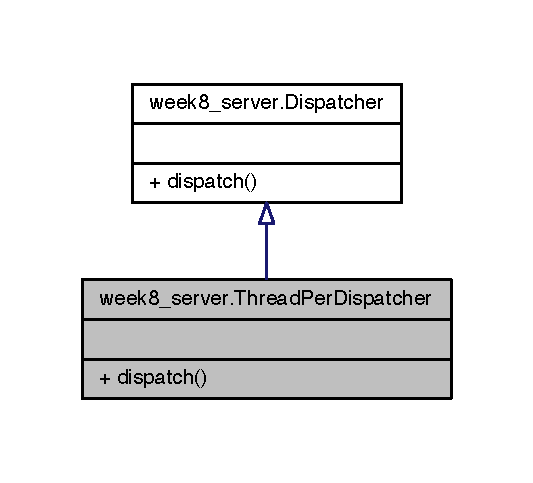
\includegraphics[width=256pt]{classweek8__server_1_1_thread_per_dispatcher__inherit__graph}
\end{center}
\end{figure}


week8\-\_\-server.\-Thread\-Per\-Dispatcher에 대한 협력 다이어그램\-:
\nopagebreak
\begin{figure}[H]
\begin{center}
\leavevmode
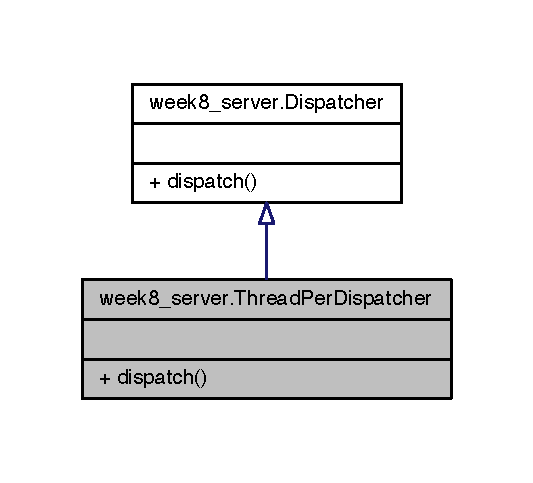
\includegraphics[width=256pt]{classweek8__server_1_1_thread_per_dispatcher__coll__graph}
\end{center}
\end{figure}
\subsection*{Public 멤버 함수}
\begin{DoxyCompactItemize}
\item 
void \hyperlink{classweek8__server_1_1_thread_per_dispatcher_acf253a1552859366b9420eb3ede8ea49}{dispatch} (Server\-Socket server\-Socket, \hyperlink{classweek8__server_1_1_handle_map}{Handle\-Map} handle\-Map)
\begin{DoxyCompactList}\small\item\em create thread for demultiplexer (handle request) \end{DoxyCompactList}\end{DoxyCompactItemize}


\subsection{상세한 설명}
dispatcher create thread for each stream 

dispatcher create thread pool and use for handle request

\begin{DoxyDate}{날짜}
2014-\/09-\/17 
\end{DoxyDate}
\begin{DoxyAuthor}{작성자}
youngkim, \href{mailto:ky200223@nhnnext.org}{\tt ky200223@nhnnext.\-org}
\end{DoxyAuthor}
create thread for each stream to handle request

\begin{DoxyDate}{날짜}
2014-\/09-\/17 
\end{DoxyDate}
\begin{DoxyAuthor}{작성자}
youngkim, \href{mailto:ky200223@nhnnext.org}{\tt ky200223@nhnnext.\-org}
\end{DoxyAuthor}
create thread pool to handle request 

Thread\-Per\-Dispatcher.\-java 파일의 24 번째 라인에서 정의되었습니다.



\subsection{멤버 함수 문서화}
\hypertarget{classweek8__server_1_1_thread_per_dispatcher_acf253a1552859366b9420eb3ede8ea49}{\index{week8\-\_\-server\-::\-Thread\-Per\-Dispatcher@{week8\-\_\-server\-::\-Thread\-Per\-Dispatcher}!dispatch@{dispatch}}
\index{dispatch@{dispatch}!week8_server::ThreadPerDispatcher@{week8\-\_\-server\-::\-Thread\-Per\-Dispatcher}}
\subsubsection[{dispatch}]{\setlength{\rightskip}{0pt plus 5cm}void week8\-\_\-server.\-Thread\-Per\-Dispatcher.\-dispatch (
\begin{DoxyParamCaption}
\item[{Server\-Socket}]{server\-Socket, }
\item[{{\bf Handle\-Map}}]{handle\-Map}
\end{DoxyParamCaption}
)}}\label{classweek8__server_1_1_thread_per_dispatcher_acf253a1552859366b9420eb3ede8ea49}


create thread for demultiplexer (handle request) 

init demultiplexer and run as thread / create thread for each request 
\begin{DoxyParams}{매개변수}
{\em server\-Socket,handle\-Map} & \\
\hline
\end{DoxyParams}
\begin{DoxyReturn}{반환값}
none 
\end{DoxyReturn}


\hyperlink{interfaceweek8__server_1_1_dispatcher_a29b5387e03751725f89de08211e638b7}{week8\-\_\-server.\-Dispatcher}를 구현.



Thread\-Per\-Dispatcher.\-java 파일의 32 번째 라인에서 정의되었습니다.


\begin{DoxyCode}
32                                                                          \{
33         \textcolor{keywordflow}{while} (\textcolor{keyword}{true}) \{
34             \textcolor{keywordflow}{try} \{
35                 Socket socket = serverSocket.accept();
36 
37                 Runnable demultiplexer = \textcolor{keyword}{new} Demultiplexer(socket, handleMap);
38                 Thread thread = \textcolor{keyword}{new} Thread(demultiplexer);
39                 thread.start();
40 
41             \} \textcolor{keywordflow}{catch} (IOException e) \{
42                 e.printStackTrace();
43             \}
44         \}
45     \}
\end{DoxyCode}


이 클래스에 대한 문서화 페이지는 다음의 파일로부터 생성되었습니다.\-:\begin{DoxyCompactItemize}
\item 
src/week8\-\_\-server/\hyperlink{_thread_per_dispatcher_8java}{Thread\-Per\-Dispatcher.\-java}\end{DoxyCompactItemize}

\hypertarget{classweek8__server_1_1_thread_pool_dispatcher}{\section{week8\-\_\-server.\-Thread\-Pool\-Dispatcher 클래스 참조}
\label{classweek8__server_1_1_thread_pool_dispatcher}\index{week8\-\_\-server.\-Thread\-Pool\-Dispatcher@{week8\-\_\-server.\-Thread\-Pool\-Dispatcher}}
}


week8\-\_\-server.\-Thread\-Pool\-Dispatcher에 대한 상속 다이어그램 \-: 
\nopagebreak
\begin{figure}[H]
\begin{center}
\leavevmode
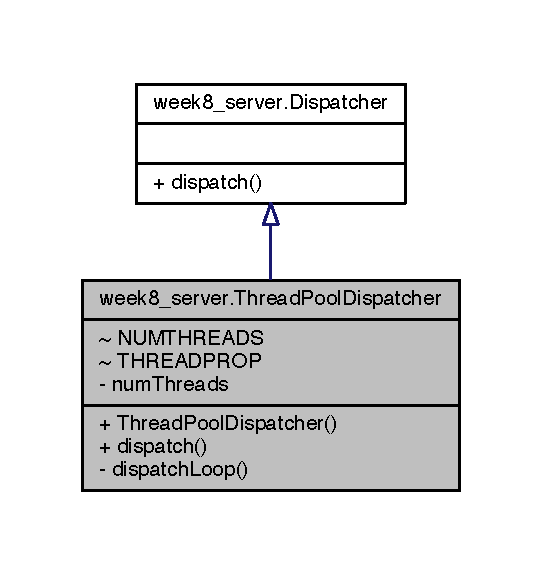
\includegraphics[width=260pt]{classweek8__server_1_1_thread_pool_dispatcher__inherit__graph}
\end{center}
\end{figure}


week8\-\_\-server.\-Thread\-Pool\-Dispatcher에 대한 협력 다이어그램\-:
\nopagebreak
\begin{figure}[H]
\begin{center}
\leavevmode
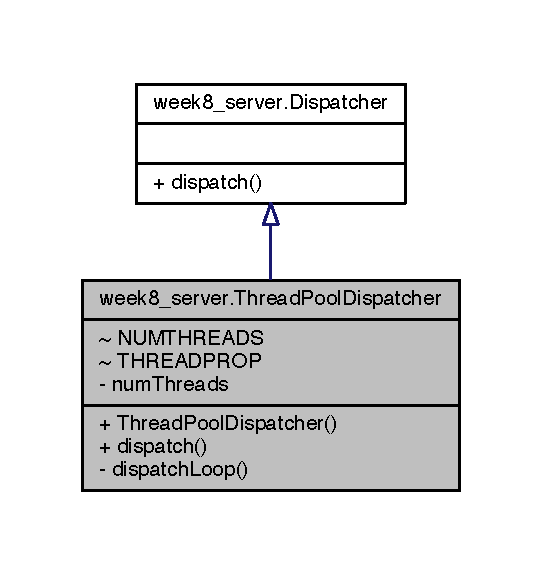
\includegraphics[width=260pt]{classweek8__server_1_1_thread_pool_dispatcher__coll__graph}
\end{center}
\end{figure}
\subsection*{Public 멤버 함수}
\begin{DoxyCompactItemize}
\item 
\hyperlink{classweek8__server_1_1_thread_pool_dispatcher_afbd2f886e943d35e97a251510d415882}{Thread\-Pool\-Dispatcher} ()
\begin{DoxyCompactList}\small\item\em constructor / set thread\-Num from system property \end{DoxyCompactList}\item 
void \hyperlink{classweek8__server_1_1_thread_pool_dispatcher_a44247cc26ed377303c2e86e00863cf6a}{dispatch} (final Server\-Socket server\-Socket, final \hyperlink{classweek8__server_1_1_handle_map}{Handle\-Map} handle\-Map)
\begin{DoxyCompactList}\small\item\em create thread pool for demultiplexer \end{DoxyCompactList}\item 
void \hyperlink{interfaceweek8__server_1_1_dispatcher_a29b5387e03751725f89de08211e638b7}{dispatch} (Server\-Socket server\-Socket, \hyperlink{classweek8__server_1_1_handle_map}{Handle\-Map} handle\-Map)
\end{DoxyCompactItemize}
\subsection*{Private 멤버 함수}
\begin{DoxyCompactItemize}
\item 
void \hyperlink{classweek8__server_1_1_thread_pool_dispatcher_a7138d250700b8e7c5840ebfe11da0e83}{dispatch\-Loop} (Server\-Socket server\-Socket, \hyperlink{classweek8__server_1_1_handle_map}{Handle\-Map} handle\-Map)
\begin{DoxyCompactList}\small\item\em excute demultiplexer (handle request) -\/ run on thread \end{DoxyCompactList}\end{DoxyCompactItemize}
\subsection*{Private 속성}
\begin{DoxyCompactItemize}
\item 
int \hyperlink{classweek8__server_1_1_thread_pool_dispatcher_af2930528df7e19e996420a857079ea69}{num\-Threads}
\end{DoxyCompactItemize}


\subsection{상세한 설명}


Thread\-Pool\-Dispatcher.\-java 파일의 24 번째 라인에서 정의되었습니다.



\subsection{생성자 \& 소멸자 문서화}
\hypertarget{classweek8__server_1_1_thread_pool_dispatcher_afbd2f886e943d35e97a251510d415882}{\index{week8\-\_\-server\-::\-Thread\-Pool\-Dispatcher@{week8\-\_\-server\-::\-Thread\-Pool\-Dispatcher}!Thread\-Pool\-Dispatcher@{Thread\-Pool\-Dispatcher}}
\index{Thread\-Pool\-Dispatcher@{Thread\-Pool\-Dispatcher}!week8_server::ThreadPoolDispatcher@{week8\-\_\-server\-::\-Thread\-Pool\-Dispatcher}}
\subsubsection[{Thread\-Pool\-Dispatcher}]{\setlength{\rightskip}{0pt plus 5cm}week8\-\_\-server.\-Thread\-Pool\-Dispatcher.\-Thread\-Pool\-Dispatcher (
\begin{DoxyParamCaption}
{}
\end{DoxyParamCaption}
)}}\label{classweek8__server_1_1_thread_pool_dispatcher_afbd2f886e943d35e97a251510d415882}


constructor / set thread\-Num from system property 


\begin{DoxyParams}{매개변수}
{\em none} & \\
\hline
\end{DoxyParams}
\begin{DoxyReturn}{반환값}
none 
\end{DoxyReturn}


Thread\-Pool\-Dispatcher.\-java 파일의 36 번째 라인에서 정의되었습니다.


\begin{DoxyCode}
36                                   \{
37         \hyperlink{classweek8__server_1_1_thread_pool_dispatcher_af2930528df7e19e996420a857079ea69}{numThreads} = Integer.parseInt(System
38                 .getProperty(THREADPROP, NUMTHREADS));
39     \}
\end{DoxyCode}


\subsection{멤버 함수 문서화}
\hypertarget{interfaceweek8__server_1_1_dispatcher_a29b5387e03751725f89de08211e638b7}{\index{week8\-\_\-server\-::\-Thread\-Pool\-Dispatcher@{week8\-\_\-server\-::\-Thread\-Pool\-Dispatcher}!dispatch@{dispatch}}
\index{dispatch@{dispatch}!week8_server::ThreadPoolDispatcher@{week8\-\_\-server\-::\-Thread\-Pool\-Dispatcher}}
\subsubsection[{dispatch}]{\setlength{\rightskip}{0pt plus 5cm}void week8\-\_\-server.\-Dispatcher.\-dispatch (
\begin{DoxyParamCaption}
\item[{Server\-Socket}]{server\-Socket, }
\item[{{\bf Handle\-Map}}]{handle\-Map}
\end{DoxyParamCaption}
)\hspace{0.3cm}{\ttfamily [inherited]}}}\label{interfaceweek8__server_1_1_dispatcher_a29b5387e03751725f89de08211e638b7}


\hyperlink{classweek8__server_1_1_thread_per_dispatcher_acf253a1552859366b9420eb3ede8ea49}{week8\-\_\-server.\-Thread\-Per\-Dispatcher}에서 구현되었습니다.

\hypertarget{classweek8__server_1_1_thread_pool_dispatcher_a44247cc26ed377303c2e86e00863cf6a}{\index{week8\-\_\-server\-::\-Thread\-Pool\-Dispatcher@{week8\-\_\-server\-::\-Thread\-Pool\-Dispatcher}!dispatch@{dispatch}}
\index{dispatch@{dispatch}!week8_server::ThreadPoolDispatcher@{week8\-\_\-server\-::\-Thread\-Pool\-Dispatcher}}
\subsubsection[{dispatch}]{\setlength{\rightskip}{0pt plus 5cm}void week8\-\_\-server.\-Thread\-Pool\-Dispatcher.\-dispatch (
\begin{DoxyParamCaption}
\item[{final Server\-Socket}]{server\-Socket, }
\item[{final {\bf Handle\-Map}}]{handle\-Map}
\end{DoxyParamCaption}
)}}\label{classweek8__server_1_1_thread_pool_dispatcher_a44247cc26ed377303c2e86e00863cf6a}


create thread pool for demultiplexer 

init demultiplexer and run as thread / create thread pool 
\begin{DoxyParams}{매개변수}
{\em server\-Socket,handle\-Map} & \\
\hline
\end{DoxyParams}
\begin{DoxyReturn}{반환값}
none 
\end{DoxyReturn}


Thread\-Pool\-Dispatcher.\-java 파일의 47 번째 라인에서 정의되었습니다.


\begin{DoxyCode}
48                                        \{
49         \textcolor{keywordflow}{for} (\textcolor{keywordtype}{int} i = 0; i < (\hyperlink{classweek8__server_1_1_thread_pool_dispatcher_af2930528df7e19e996420a857079ea69}{numThreads} - 1); i++) \{
50             Thread thread = \textcolor{keyword}{new} Thread() \{
51                 \textcolor{keyword}{public} \textcolor{keywordtype}{void} run() \{
52                     \hyperlink{classweek8__server_1_1_thread_pool_dispatcher_a7138d250700b8e7c5840ebfe11da0e83}{dispatchLoop}(serverSocket, handleMap);
53                 \}
54             \};
55             thread.start();
56             System.out.println(\textcolor{stringliteral}{"Created and started Thread = "}
57                     + thread.getName());
58         \}
59 
60         \hyperlink{classweek8__server_1_1_thread_pool_dispatcher_a7138d250700b8e7c5840ebfe11da0e83}{dispatchLoop}(serverSocket, handleMap);
61     \}
\end{DoxyCode}


이 함수 내부에서 호출하는 함수들에 대한 그래프입니다.\-:
\nopagebreak
\begin{figure}[H]
\begin{center}
\leavevmode
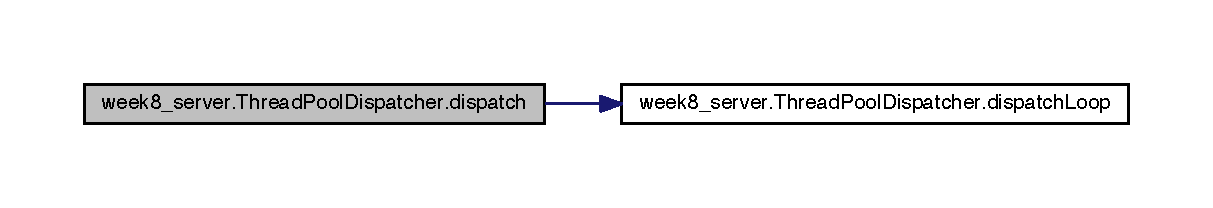
\includegraphics[width=350pt]{classweek8__server_1_1_thread_pool_dispatcher_a44247cc26ed377303c2e86e00863cf6a_cgraph}
\end{center}
\end{figure}


\hypertarget{classweek8__server_1_1_thread_pool_dispatcher_a7138d250700b8e7c5840ebfe11da0e83}{\index{week8\-\_\-server\-::\-Thread\-Pool\-Dispatcher@{week8\-\_\-server\-::\-Thread\-Pool\-Dispatcher}!dispatch\-Loop@{dispatch\-Loop}}
\index{dispatch\-Loop@{dispatch\-Loop}!week8_server::ThreadPoolDispatcher@{week8\-\_\-server\-::\-Thread\-Pool\-Dispatcher}}
\subsubsection[{dispatch\-Loop}]{\setlength{\rightskip}{0pt plus 5cm}void week8\-\_\-server.\-Thread\-Pool\-Dispatcher.\-dispatch\-Loop (
\begin{DoxyParamCaption}
\item[{Server\-Socket}]{server\-Socket, }
\item[{{\bf Handle\-Map}}]{handle\-Map}
\end{DoxyParamCaption}
)\hspace{0.3cm}{\ttfamily [private]}}}\label{classweek8__server_1_1_thread_pool_dispatcher_a7138d250700b8e7c5840ebfe11da0e83}


excute demultiplexer (handle request) -\/ run on thread 


\begin{DoxyParams}{매개변수}
{\em server\-Socket,handle\-Map} & \\
\hline
\end{DoxyParams}
\begin{DoxyReturn}{반환값}
none 
\end{DoxyReturn}


Thread\-Pool\-Dispatcher.\-java 파일의 68 번째 라인에서 정의되었습니다.


\begin{DoxyCode}
68                                                                               \{
69         \textcolor{keywordflow}{while} (\textcolor{keyword}{true}) \{
70             \textcolor{keywordflow}{try} \{
71                 Socket socket = serverSocket.accept();
72                 Runnable demultiplexer = \textcolor{keyword}{new} Demultiplexer(socket, handleMap);
73                 demultiplexer.run();
74             \} \textcolor{keywordflow}{catch} (IOException e) \{
75                 e.printStackTrace();
76             \}
77         \}
78     \}
\end{DoxyCode}


이 함수를 호출하는 함수들에 대한 그래프입니다.\-:
\nopagebreak
\begin{figure}[H]
\begin{center}
\leavevmode
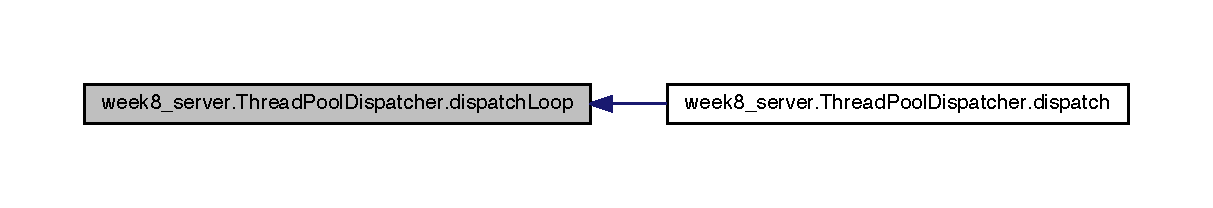
\includegraphics[width=350pt]{classweek8__server_1_1_thread_pool_dispatcher_a7138d250700b8e7c5840ebfe11da0e83_icgraph}
\end{center}
\end{figure}




\subsection{멤버 데이타 문서화}
\hypertarget{classweek8__server_1_1_thread_pool_dispatcher_af2930528df7e19e996420a857079ea69}{\index{week8\-\_\-server\-::\-Thread\-Pool\-Dispatcher@{week8\-\_\-server\-::\-Thread\-Pool\-Dispatcher}!num\-Threads@{num\-Threads}}
\index{num\-Threads@{num\-Threads}!week8_server::ThreadPoolDispatcher@{week8\-\_\-server\-::\-Thread\-Pool\-Dispatcher}}
\subsubsection[{num\-Threads}]{\setlength{\rightskip}{0pt plus 5cm}int week8\-\_\-server.\-Thread\-Pool\-Dispatcher.\-num\-Threads\hspace{0.3cm}{\ttfamily [private]}}}\label{classweek8__server_1_1_thread_pool_dispatcher_af2930528df7e19e996420a857079ea69}


Thread\-Pool\-Dispatcher.\-java 파일의 29 번째 라인에서 정의되었습니다.



이 클래스에 대한 문서화 페이지는 다음의 파일로부터 생성되었습니다.\-:\begin{DoxyCompactItemize}
\item 
src/week8\-\_\-server/\hyperlink{_thread_pool_dispatcher_8java}{Thread\-Pool\-Dispatcher.\-java}\end{DoxyCompactItemize}

\chapter{파일 문서화}
\hypertarget{_demultiplexer_8java}{\section{src/week8\-\_\-server/\-Demultiplexer.java 파일 참조}
\label{_demultiplexer_8java}\index{src/week8\-\_\-server/\-Demultiplexer.\-java@{src/week8\-\_\-server/\-Demultiplexer.\-java}}
}


route request with header info to each handler  


\subsection*{클래스}
\begin{DoxyCompactItemize}
\item 
class \hyperlink{classweek8__server_1_1_demultiplexer}{week8\-\_\-server.\-Demultiplexer}
\begin{DoxyCompactList}\small\item\em route request with header info to each handler \end{DoxyCompactList}\end{DoxyCompactItemize}
\subsection*{패키지}
\begin{DoxyCompactItemize}
\item 
package \hyperlink{namespaceweek8__server}{week8\-\_\-server}
\begin{DoxyCompactList}\small\item\em project package \end{DoxyCompactList}\end{DoxyCompactItemize}


\subsection{상세한 설명}
route request with header info to each handler \begin{DoxyAuthor}{작성자}
youngkim 
\end{DoxyAuthor}


\hyperlink{_demultiplexer_8java_source}{Demultiplexer.\-java} 파일에서 정의되었습니다.


\hypertarget{_dispatcher_8java}{\section{src/week8\-\_\-server/\-Dispatcher.java 파일 참조}
\label{_dispatcher_8java}\index{src/week8\-\_\-server/\-Dispatcher.\-java@{src/week8\-\_\-server/\-Dispatcher.\-java}}
}


dispatcher interface  


\subsection*{클래스}
\begin{DoxyCompactItemize}
\item 
interface \hyperlink{interfaceweek8__server_1_1_dispatcher}{week8\-\_\-server.\-Dispatcher}
\end{DoxyCompactItemize}
\subsection*{패키지}
\begin{DoxyCompactItemize}
\item 
package \hyperlink{namespaceweek8__server}{week8\-\_\-server}
\begin{DoxyCompactList}\small\item\em project package \end{DoxyCompactList}\end{DoxyCompactItemize}


\subsection{상세한 설명}
dispatcher interface \begin{DoxyAuthor}{작성자}
youngkim 
\end{DoxyAuthor}


\hyperlink{_dispatcher_8java_source}{Dispatcher.\-java} 파일에서 정의되었습니다.


\hypertarget{_event_handler_8java}{\section{src/week8\-\_\-server/\-Event\-Handler.java 파일 참조}
\label{_event_handler_8java}\index{src/week8\-\_\-server/\-Event\-Handler.\-java@{src/week8\-\_\-server/\-Event\-Handler.\-java}}
}


Event\-Handler interface.  


\subsection*{클래스}
\begin{DoxyCompactItemize}
\item 
interface \hyperlink{interfaceweek8__server_1_1_event_handler}{week8\-\_\-server.\-Event\-Handler}
\end{DoxyCompactItemize}
\subsection*{패키지}
\begin{DoxyCompactItemize}
\item 
package \hyperlink{namespaceweek8__server}{week8\-\_\-server}
\begin{DoxyCompactList}\small\item\em project package \end{DoxyCompactList}\end{DoxyCompactItemize}


\subsection{상세한 설명}
Event\-Handler interface. \begin{DoxyAuthor}{작성자}
youngkim 
\end{DoxyAuthor}


\hyperlink{_event_handler_8java_source}{Event\-Handler.\-java} 파일에서 정의되었습니다.


\hypertarget{_handle_map_8java}{\section{src/week8\-\_\-server/\-Handle\-Map.java 파일 참조}
\label{_handle_map_8java}\index{src/week8\-\_\-server/\-Handle\-Map.\-java@{src/week8\-\_\-server/\-Handle\-Map.\-java}}
}


Handle\-Map for store handler.  


\subsection*{클래스}
\begin{DoxyCompactItemize}
\item 
class \hyperlink{classweek8__server_1_1_handle_map}{week8\-\_\-server.\-Handle\-Map}
\end{DoxyCompactItemize}
\subsection*{패키지}
\begin{DoxyCompactItemize}
\item 
package \hyperlink{namespaceweek8__server}{week8\-\_\-server}
\begin{DoxyCompactList}\small\item\em project package \end{DoxyCompactList}\end{DoxyCompactItemize}


\subsection{상세한 설명}
Handle\-Map for store handler. \begin{DoxyAuthor}{작성자}
youngkim 
\end{DoxyAuthor}


\hyperlink{_handle_map_8java_source}{Handle\-Map.\-java} 파일에서 정의되었습니다.


\hypertarget{_handler_list_data_8java}{\section{src/week8\-\_\-server/\-Handler\-List\-Data.java 파일 참조}
\label{_handler_list_data_8java}\index{src/week8\-\_\-server/\-Handler\-List\-Data.\-java@{src/week8\-\_\-server/\-Handler\-List\-Data.\-java}}
}


class for simpleframework  


\subsection*{클래스}
\begin{DoxyCompactItemize}
\item 
class \hyperlink{classweek8__server_1_1_handler_list_data}{week8\-\_\-server.\-Handler\-List\-Data}
\end{DoxyCompactItemize}
\subsection*{패키지}
\begin{DoxyCompactItemize}
\item 
package \hyperlink{namespaceweek8__server}{week8\-\_\-server}
\begin{DoxyCompactList}\small\item\em project package \end{DoxyCompactList}\end{DoxyCompactItemize}


\subsection{상세한 설명}
class for simpleframework \begin{DoxyAuthor}{작성자}
youngkim 
\end{DoxyAuthor}


\hyperlink{_handler_list_data_8java_source}{Handler\-List\-Data.\-java} 파일에서 정의되었습니다.


\hypertarget{_reactor_8java}{\section{src/week8\-\_\-server/\-Reactor.java 파일 참조}
\label{_reactor_8java}\index{src/week8\-\_\-server/\-Reactor.\-java@{src/week8\-\_\-server/\-Reactor.\-java}}
}


contains method for reactor server, start / get,set handler  


\subsection*{클래스}
\begin{DoxyCompactItemize}
\item 
class \hyperlink{classweek8__server_1_1_reactor}{week8\-\_\-server.\-Reactor}
\begin{DoxyCompactList}\small\item\em contains method for reactor server, start / get,set handler \end{DoxyCompactList}\end{DoxyCompactItemize}
\subsection*{패키지}
\begin{DoxyCompactItemize}
\item 
package \hyperlink{namespaceweek8__server}{week8\-\_\-server}
\begin{DoxyCompactList}\small\item\em project package \end{DoxyCompactList}\end{DoxyCompactItemize}


\subsection{상세한 설명}
contains method for reactor server, start / get,set handler \begin{DoxyAuthor}{작성자}
youngkim 
\end{DoxyAuthor}


\hyperlink{_reactor_8java_source}{Reactor.\-java} 파일에서 정의되었습니다.


\hypertarget{_server_initializer_8java}{\section{src/week8\-\_\-server/\-Server\-Initializer.java 파일 참조}
\label{_server_initializer_8java}\index{src/week8\-\_\-server/\-Server\-Initializer.\-java@{src/week8\-\_\-server/\-Server\-Initializer.\-java}}
}


Contains main method to run server / logger example.  


\subsection*{클래스}
\begin{DoxyCompactItemize}
\item 
class \hyperlink{classweek8__server_1_1_server_initializer}{week8\-\_\-server.\-Server\-Initializer}
\begin{DoxyCompactList}\small\item\em Initializer class for Reactor-\/\-Thread using server. \end{DoxyCompactList}\end{DoxyCompactItemize}
\subsection*{패키지}
\begin{DoxyCompactItemize}
\item 
package \hyperlink{namespaceweek8__server}{week8\-\_\-server}
\begin{DoxyCompactList}\small\item\em project package \end{DoxyCompactList}\end{DoxyCompactItemize}


\subsection{상세한 설명}
Contains main method to run server / logger example. \begin{DoxyAuthor}{작성자}
youngkim 
\end{DoxyAuthor}


\hyperlink{_server_initializer_8java_source}{Server\-Initializer.\-java} 파일에서 정의되었습니다.


\hypertarget{_server_list_data_8java}{\section{src/week8\-\_\-server/\-Server\-List\-Data.java 파일 참조}
\label{_server_list_data_8java}\index{src/week8\-\_\-server/\-Server\-List\-Data.\-java@{src/week8\-\_\-server/\-Server\-List\-Data.\-java}}
}


class for simpleframework  


\subsection*{클래스}
\begin{DoxyCompactItemize}
\item 
class \hyperlink{classweek8__server_1_1_server_list_data}{week8\-\_\-server.\-Server\-List\-Data}
\end{DoxyCompactItemize}
\subsection*{패키지}
\begin{DoxyCompactItemize}
\item 
package \hyperlink{namespaceweek8__server}{week8\-\_\-server}
\begin{DoxyCompactList}\small\item\em project package \end{DoxyCompactList}\end{DoxyCompactItemize}


\subsection{상세한 설명}
class for simpleframework \begin{DoxyAuthor}{작성자}
youngkim 
\end{DoxyAuthor}


\hyperlink{_server_list_data_8java_source}{Server\-List\-Data.\-java} 파일에서 정의되었습니다.


\hypertarget{_stream_say_hello_event_handler_8java}{\section{src/week8\-\_\-server/\-Stream\-Say\-Hello\-Event\-Handler.java 파일 참조}
\label{_stream_say_hello_event_handler_8java}\index{src/week8\-\_\-server/\-Stream\-Say\-Hello\-Event\-Handler.\-java@{src/week8\-\_\-server/\-Stream\-Say\-Hello\-Event\-Handler.\-java}}
}
\subsection*{클래스}
\begin{DoxyCompactItemize}
\item 
class \hyperlink{classweek8__server_1_1_stream_say_hello_event_handler}{week8\-\_\-server.\-Stream\-Say\-Hello\-Event\-Handler}
\begin{DoxyCompactList}\small\item\em route request with header info to each handler \end{DoxyCompactList}\end{DoxyCompactItemize}
\subsection*{패키지}
\begin{DoxyCompactItemize}
\item 
package \hyperlink{namespaceweek8__server}{week8\-\_\-server}
\begin{DoxyCompactList}\small\item\em project package \end{DoxyCompactList}\end{DoxyCompactItemize}

\hypertarget{_stream_update_profile_event_handler_8java}{\section{src/week8\-\_\-server/\-Stream\-Update\-Profile\-Event\-Handler.java 파일 참조}
\label{_stream_update_profile_event_handler_8java}\index{src/week8\-\_\-server/\-Stream\-Update\-Profile\-Event\-Handler.\-java@{src/week8\-\_\-server/\-Stream\-Update\-Profile\-Event\-Handler.\-java}}
}


handle request that header is 0x6001  


\subsection*{클래스}
\begin{DoxyCompactItemize}
\item 
class \hyperlink{classweek8__server_1_1_stream_update_profile_event_handler}{week8\-\_\-server.\-Stream\-Update\-Profile\-Event\-Handler}
\begin{DoxyCompactList}\small\item\em route request with header info to each handler \end{DoxyCompactList}\end{DoxyCompactItemize}
\subsection*{패키지}
\begin{DoxyCompactItemize}
\item 
package \hyperlink{namespaceweek8__server}{week8\-\_\-server}
\begin{DoxyCompactList}\small\item\em project package \end{DoxyCompactList}\end{DoxyCompactItemize}


\subsection{상세한 설명}
handle request that header is 0x6001 \begin{DoxyAuthor}{작성자}
youngkim 
\end{DoxyAuthor}


\hyperlink{_stream_update_profile_event_handler_8java_source}{Stream\-Update\-Profile\-Event\-Handler.\-java} 파일에서 정의되었습니다.


\hypertarget{_test_client_8java}{\section{src/week8\-\_\-server/\-Test\-Client.java 파일 참조}
\label{_test_client_8java}\index{src/week8\-\_\-server/\-Test\-Client.\-java@{src/week8\-\_\-server/\-Test\-Client.\-java}}
}


outputstream data for test  


\subsection*{클래스}
\begin{DoxyCompactItemize}
\item 
class \hyperlink{classweek8__server_1_1_test_client}{week8\-\_\-server.\-Test\-Client}
\begin{DoxyCompactList}\small\item\em outputstream data for test \end{DoxyCompactList}\end{DoxyCompactItemize}
\subsection*{패키지}
\begin{DoxyCompactItemize}
\item 
package \hyperlink{namespaceweek8__server}{week8\-\_\-server}
\begin{DoxyCompactList}\small\item\em project package \end{DoxyCompactList}\end{DoxyCompactItemize}


\subsection{상세한 설명}
outputstream data for test \begin{DoxyAuthor}{작성자}
youngkim 
\end{DoxyAuthor}


\hyperlink{_test_client_8java_source}{Test\-Client.\-java} 파일에서 정의되었습니다.


\hypertarget{_thread_per_dispatcher_8java}{\section{src/week8\-\_\-server/\-Thread\-Per\-Dispatcher.java 파일 참조}
\label{_thread_per_dispatcher_8java}\index{src/week8\-\_\-server/\-Thread\-Per\-Dispatcher.\-java@{src/week8\-\_\-server/\-Thread\-Per\-Dispatcher.\-java}}
}


dispatcher create thread for each stream  


\subsection*{클래스}
\begin{DoxyCompactItemize}
\item 
class \hyperlink{classweek8__server_1_1_thread_per_dispatcher}{week8\-\_\-server.\-Thread\-Per\-Dispatcher}
\begin{DoxyCompactList}\small\item\em dispatcher create thread for each stream \end{DoxyCompactList}\end{DoxyCompactItemize}
\subsection*{패키지}
\begin{DoxyCompactItemize}
\item 
package \hyperlink{namespaceweek8__server}{week8\-\_\-server}
\begin{DoxyCompactList}\small\item\em project package \end{DoxyCompactList}\end{DoxyCompactItemize}


\subsection{상세한 설명}
dispatcher create thread for each stream \begin{DoxyAuthor}{작성자}
youngkim 
\end{DoxyAuthor}


\hyperlink{_thread_per_dispatcher_8java_source}{Thread\-Per\-Dispatcher.\-java} 파일에서 정의되었습니다.


\hypertarget{_thread_pool_dispatcher_8java}{\section{src/week8\-\_\-server/\-Thread\-Pool\-Dispatcher.java 파일 참조}
\label{_thread_pool_dispatcher_8java}\index{src/week8\-\_\-server/\-Thread\-Pool\-Dispatcher.\-java@{src/week8\-\_\-server/\-Thread\-Pool\-Dispatcher.\-java}}
}


dispatcher create thread pool and use for handle request  


\subsection*{클래스}
\begin{DoxyCompactItemize}
\item 
class \hyperlink{classweek8__server_1_1_thread_pool_dispatcher}{week8\-\_\-server.\-Thread\-Pool\-Dispatcher}
\end{DoxyCompactItemize}
\subsection*{패키지}
\begin{DoxyCompactItemize}
\item 
package \hyperlink{namespaceweek8__server}{week8\-\_\-server}
\begin{DoxyCompactList}\small\item\em project package \end{DoxyCompactList}\end{DoxyCompactItemize}


\subsection{상세한 설명}
dispatcher create thread pool and use for handle request \begin{DoxyAuthor}{작성자}
youngkim 
\end{DoxyAuthor}


\hyperlink{_thread_pool_dispatcher_8java_source}{Thread\-Pool\-Dispatcher.\-java} 파일에서 정의되었습니다.


%--- End generated contents ---

% Index
\newpage
\phantomsection
\addcontentsline{toc}{chapter}{색인}
\printindex

\end{document}
